\chapter{Phonetik}
\label{kap:Phonetik}

In den vorangegangenen Kapiteln ging es um größere und kleinere Einheiten der Sprache, mit denen wir allerdings immer eine Bedeutung verknüpfen konnten. Im aktuellen Kapitel zur Phonetik widmen wir uns kleineren Einheiten der Sprache, denen wir für sich genommen keine Bedeutung mehr zuordnen können. Diese Einheiten sind die Laute. Ein weiterer Unterschied zu den vorangegangen Kapiteln besteht darin, dass wir uns im aktuellen Kapitel speziell mit der gesprochenen Sprache beschäftigen, während es in den vorangegangenen Kapiteln immer sowohl um gesprochene als auch um geschriebene Sprache ging. Trotzdem ist das aktuelle Kapitel auch für das Verständnis der geschriebenen Sprache relevant, weil das deutsche Schriftsystem alphabetisch ist und deshalb auf einer Zuordnung von bestimmten Lauten (den sogenannten Phonemen, vgl. Abschnitt~\ref{sec:Allophone}) zu Schriftzeichen (den sogenannten Graphemen, vgl. Abschnitt~\ref{sec:BuchstabenGrapheme}) basiert. 

Phonetische Fragestellungen sind etwa:
\begin{itemize}
    \item Wie werden Laute von Sprecherinnen und Sprechern produziert?
    \item Welche Laute gibt es in den Sprachen der Welt oder in einer bestimmten Sprache?
    \item Warum sind bestimmte Laute seltener als andere? Der Laut \textipa{[g]} ist, wie \citet[719--721]{Maddieson2003} zeigt, zum Beispiel seltener als \textipa{[k]} .
\end{itemize}

Während die Schreibung des Deutschen über ein amtliches Regelwerk festgelegt ist, gibt es für die Lautung keine solch klar definierte Norm. 1898 gab es mit der Siebs-Kommission jedoch auch bezüglich der Lautung Bemühungen, zu einer festen Norm zu kommen, die für die Verwendung am Theater und an den Schulen gedacht war \citep[31f]{DudenAussprache2023}. Diese Lautung orientierte sich an der im Norden Deutschlands gesprochenen sogenannten Hochlautung, da diese Aussprache damals das größte Prestige besaß. Bis heute wird die Duden-Aussprachenorm von Berufssprechern umgesetzt und genießt darüber hinaus eine weite Akzeptanz. Im Gegensatz zur Schreibung wird sie aber von weiten Teilen der Bevölkerung nicht umgesetzt. Auch für die Schweiz und Österreich gibt es mit \citet{HoveHaas2009} und \citet{Wiesinger2009} definierte Standards. Aber auch in diesen Regionen wird diese Lautung von den Sprecherinnen und Sprechern nicht unbedingt aktiv umgesetzt. 

In diesem Buch werden wir einen Fokus auf die norddeutsche Standardlautung legen, die durch das \citet{DudenAussprache2023} definiert ist. Auf die anderen Varietäten werden wir aber immer wieder hinweisen, denn es ist für die Alphabetisierung von Kindern wichtig zu wissen, inwiefern die Aussprache der Kinder von der -- schriftnahen -- Standardlautung abweicht.

Für angehende Lehrkräfte sind phonetische Grundkenntnisse wichtig, weil man mittels dieser Kenntnisse ein Bewusstsein für die Unterschiede zwischen Lautung und Schreibung entwickeln kann. Betrachten wir dazu eine Erstklässlerschreibung:

\ea [*]{mont}\label{ea:mont} 
\z

Gemeint ist hier das Wort \textit{Mund}. Um dieses Wort zu verschriften, hat das Kind das Wort vermutlich in der Varietät, die es erworben hat, langsam gesprochen und vier Laute extrahiert: \textipa{[m]}, \textipa{[o]}, \textipa{[n]} und \textipa{[t]}. Dass das Wort mit einem Großbuchstaben geschrieben werden muss, kann man nicht hören, deshalb schreibt das Kind klein. Schwieriger nachzuvollziehen ist für kompetente Schreiberinnen und Schreiber die Motivation für das \textipa{[o]}. Wenn Sprecherinnen und Sprecher des norddeutschen Standards das Wort jedoch langsam sprechen, fällt auf, dass der Vokal, der dort gebildet wird, in gedehnter Form tatsächlich dem \textipa{[o]} sehr ähnlich ist. Er klingt in etwa wie das \textipa{[o]} in \textit{Mond}. Offenbar ist das, was wir aus der Schule als \gqq{kurzes u} kennen, zumindest im norddeutschen Standard dem langen \textipa{[o]} ähnlicher als dem langen \textipa{[u]}. Schließlich schreibt das Kind nach dem \textipa{[n]} <t> statt <d>, weil dort eben kein \textipa{[d]} gesprochen wird. 

Wissen über die Phonetik des Deutschen und seiner Varietäten hilft also dabei, Fehlschreibungen von Lernenden zu verstehen. Mittels dieses Wissens kann man unterscheiden, ob ein bestimmter Aspekt einer Schreibung aus der Lautung überhaupt abgeleitet werden kann oder nicht.
\is{IPA}

Gesprochene Sprache kann konserviert werden, etwa durch eine Mikrophonaufnahme. Alternativ kann sie mittels des \textit{IPA}, des internationalen phonetischen Alphabets \citep{IPA1999}, \textit{transkribiert} (aufgeschrieben) werden. Das Wort \textit{Mund} kann wie folgt transkribiert werden: \textipa{[mUnt]}. 

Das IPA bietet die Möglichkeit, Äußerungen unterschiedlich genau zu notieren. Wie bei \textipa{[mUnt]} kann man sich beispielsweise darauf beschränken, nur bedeutungsunterscheidende Laute einer Varietät zu transkribieren (\textit{weite Transkription}).\is{Transkription!weit}
 Das ist sinnvoll, wenn wir etwa auf den Unterschied zwischen der Lautung und der Schreibung eines Wortes hinweisen wollen. Wollen wir etwa verdeutlichen, dass das Wort \textit{Spaß} am Anfang mit \textipa{[S]} gesprochen wird, obwohl man <s> schreibt, bietet sich diese Transkription an: \textipa{[Spa:s]}. Die eckigen Klammern zeigen hier an, dass die Zeichen zwischen ihnen als IPA (also nicht orthografisch) zu lesen sind. Wenn wir explizit eine Schreibung meinen, setzen wir das Wort hingegen in spitze Klammern: <Spaß>.

Man\is{Transkription!eng} kann das IPA auch verwenden, um Äußerungen sehr detailreich zu transkribieren (\textit{enge Transkription}). Beispielsweise könnten wir pathologische Sprache -- etwa einen Sigmatismus (Lispeln) -- dadurch kennzeichnen, dass wir das \textipa{[s]} mit einem zusätzlichen Zeichen für \textit{dental} kennzeichnen: \textipa{[\textsubbridge{s}]}.\footnote{Eine Übersicht über das IPA-Zeicheninventar findet man hier:  \url{https://www.internationalphoneticassociation.org/sites/default/files/IPA_Kiel_2015.pdf} (Zugriff am 09.09.2025). Wenn man Texte in IPA tippen will, bieten sich folgende Seiten an: \url{https://ipa.typeit.org/full/} oder \url{https://westonruter.github.io/ipa-chart/keyboard/} (Zugriff am 09.09.2025)}

In diesem Kapitel werden alle für den norddeutschen Standard relevanten Zeichen des IPA vorgestellt. Leserinnen und Leser ohne Vorkenntnisse zum IPA werden zu Beginn des Kapitels Transkriptionen finden, die sie noch nicht -- oder noch nicht vollständig -- lesen können. Über das Kapitel hinweg werden die Transkriptionen aber auch für diese Leserinnen und Leser immer verständlicher werden.

Zu Beginn des Kapitels, in Abschnitt~\ref{sec:Vokaltrakt}, wird der Artikulationsapparat vorgestellt. Im darauf folgenden Abschnitt~\ref{section:betonte_unbetonte_Silben} geht es um die Unterscheidung zwischen betonten und unbetonten Silben. In Abschnitt~\ref{sec:KonsonantenundVokale} werden Unterscheidungsmöglichkeiten zwischen Konsonanten und Vokalen diskutiert. Daran anschließend wird in Abschnitt~\ref{sec:Konsonanten} das Konsonanteninventar betrachtet und in Abschnitt~\ref{sec:Vokale} das Vokalinventar. Den Abschluss des Kapitels bilden wieder Übungen zum Thema.


\section{Der Vokaltrakt und die Stimmtonerzeugung}\label{sec:Vokaltrakt}\is{Vokaltrakt}

Die Lautbildung findet im \textit{Vokaltrakt} statt. Das ist der mit Luft gefüllte Bereich vom Kehlkopf bis zu den Lippen. Abbildung~\ref{Abb:Vokaltrakt} zeigt eine magnetresonanztomographische Aufnahme eines Sprechers bei der Produktion des Vokals \textipa{[a]}. Dargestellt ist der mittsagitale Bereich, also die Ebene genau in der Mitte des Kopfes. Die Nase und die Lippen erkennt man links in der Abbildung, den Nacken rechts. Regionen mit wenig Wasser -- etwa Luft, Knochen und Zähne -- sind schwarz dargestellt. Der gesamte Vokaltrakt (Rachen und Mundhöhle) ist daher zu großen Teilen schwarz. Regionen mit viel Wasser (etwa das Fettgewebe im Nacken) sind in schwarz-weiß-Darstellungen dunkelgrau, in Farbdarstellungen rot dargestellt. Muskelgewebe hat weniger Wasser als Fettgewebe und ist deshalb hellgrau (in Farbdarstellungen grün oder gelb) dargestellt.


\begin{figure}
    \centering
    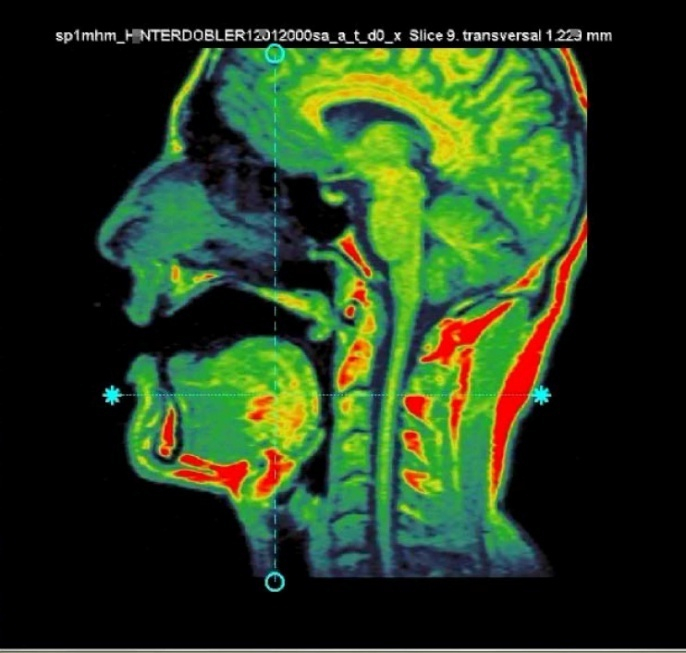
\includegraphics[]{figures/mrt_a.jpg}
    \caption{Vokaltrakt eines Sprechers in der Mittsagittalen. Quelle: Phil Hoole, Institut für Phonetik und Sprachverarbeitung, Ludwig-Maximilians-Universität München.}
    \label{Abb:Vokaltrakt}
\end{figure}


Man kann sich den Vokaltrakt als gekrümmtes Rohr vorstellen, welches vom Sprachschall passiert wird. Um unterschiedliche Laute zu produzieren, werden Verengungen, Verschlüsse oder einfach Veränderungen des Durchmessers an bestimmten Stellen realisiert. In Abbildung~\ref{Abb:Vokaltrakt} gibt es beispielsweise eine Verengung im Rachenraum, während der horizontal liegende Bereich des Vokaltrakts (die Mundhöhle) offen ist.

Im Hals, etwas unterhalb des Kinns, befindet sich der \is{Kehlkopf}Kehlkopf. Im Kehlkopf gibt es zwei Häutchen, die \is{Stimmlippen}\textit{Stimmlippen}.\footnote{Die Stimmlippen werden auch als \textit{Stimmbänder} bezeichnet. Der Begriff ist jedoch irreführend, weil er suggeriert, dass die Stimmlippen wie Gitarrensaiten schwingen.} Beim Atmen werden die Stimmlippen weit voneinander entfernt gehalten, sodass die Luft entweder aus dem Vokaltrakt in die Lunge fließt (beim Einatmen) oder in die umgekehrte Richtung aus der Lunge in den Vokaltrakt (beim Ausatmen). Die Lücke zwischen den Stimmlippen, durch die die Luft fließt, nennt man \textit{Glottis}.\is{Glottis}

Beim \is{Stimmtonerzeugung} Sprechen atmet man in der Regel aus.\footnote{Ausnahmen bilden die ingressiven Laute, bei denen die Luft in Richtung Lunge fließt, und die Clicks (Schnalzlaute), die mit oralem Luftstrommechanismus produziert werden. Bei Interesse empfehlen wir dazu \citet[4.1.9--4.1.10]{Pompino-Marschall2020}. Ingressive Laute gibt es im Deutschen nicht, aber im Hausa, einer tschadischen Sprache, oder auch im Zulu, welches in Südafrika gesprochen wird. Auch Clicks sind im Deutschen keine Phoneme, aber sie existieren in den Khoisansprachen, etwa !Xu. Zulu verfügt ebenfalls über einen Click \citep{UPSIDdatabase}.} Dabei kann mit den Stimmlippen Stimmton erzeugt werden. Die Stimmlippen werden dazu so positioniert, dass sie sich berühren und somit die Luftröhre verschließen. Gleichzeitig strömt Luft aus der Lunge in Richtung Vokaltrakt und erzeugt Druck unter den geschlossenen Stimmlippen. Ist der subglottale Druck (der Druck unter den Stimmlippen)  höher als der supraglottale Druck (der Druck über den Stimmlippen), werden die Stimmlippen aufgesprengt. In diesem Moment kommt es zum sogenannten\is{Bernoulli-Effekt} Bernoulli-Effekt, einem Sogeffekt senkrecht zur Fließrichtung der Luft \citep[32--34, 306]{Pompino-Marschall2020}. Durch diesen Effekt schließen sich die Stimmlippen wieder. Da aus der Lunge jedoch weiter Luft Richtung Vokaltrakt fließt, wiederholt sich dieser Prozess: Der Druck unter der Glottis steigt, die Glottis wird aufgesprengt und schließt sich wieder. Die periodischen Luftdruckunterschiede, die dabei entstehen, nehmen wir als Stimmton wahr.

Besser vorstellbar wird dieser Prozess des Öffnens und Schließens, wenn man ihn an einer Stelle produziert, wo er sichtbar ist, etwa mit den Lippen. Dazu schließt man die Lippen locker und versucht, hindurchzupusten. Die Lippen fangen an, sich periodisch zu öffnen und zu schließen.

Die Geschwindigkeit, mit der sich die Stimmlippen öffnen und schließen, ist einerseits von den anatomischen Gegebenheiten abhängig, kann aber andererseits auch von Sprecherinnen und Sprechern beeinflusst werden. Erwachsene Männer haben im Durchschnitt längere Stimmlippen als erwachsene Frauen. Die Stimmlippen von Kindern sind noch kürzer als die von weiblichen Erwachsenen. Wenn die Stimmlippen länger sind, dauert der oben beschriebene Zyklus von Öffnung und Schließung der Stimmlippen (unter ansonsten gleichen Bedingungen) länger. Männerstimmen öffnen und schließen sich deshalb beim Sprechen etwa 120 mal in der Sekunde (man spricht dann von einer \textit{Grundfrequenz} von 120 Hertz). Frauenstimmen schwingen laut \citet{TraunmuellerEriksson1994} im Mittel knapp doppelt so schnell (etwa 200 mal in der Sekunde) und sind deshalb knapp eine Oktave höher.\footnote{Eine Oktave entspricht einer Verdopplung der Grundfrequenz.} Kinderstimmen können, wie \citet{Reubold2012} zeigt, durch die geringere Länge der Stimmlippen noch deutlich höher sein als Frauenstimmen.

Unabhängig von ihren unterschiedlichen biologischen Voraussetzungen können Sprecherinnen und Sprecher die Stimmhöhe variieren, etwa beim Singen, aber auch beim Sprechen. \citet{Fry1958} zeigt, dass betonte Silben im Allgemeinen mit etwas höherer Grundfrequenz produziert werden als unbetonte. Um einen höheren Stimmton zu produzieren, spannen Sprecherinnen und Sprecher die Stimmlippen an; für eine tiefere Stimme lockern sie sie.

\section{Betonte und unbetonte Silben}\label{section:betonte_unbetonte_Silben}
\is{Betonung}
\is{Akzent!Hauptakzent}
\is{Akzent!Wortakzent}
Im Deutschen hat jedes Wort eine Silbe, die besonders prominent ist. Man nennt diese Silbe die \textit{betonte Silbe}, die Silbe mit dem \textit{Wortakzent} oder die Silbe mit dem \textit{Hauptakzent}. Wenn ein Wort aus nur einer einzigen Silbe besteht, trägt diese Silbe den Hauptakzent. In den folgenden Beispielen ist die betonte Silbe in der orthografischen Form durch Großbuchstaben markiert.

Einige Wörter unterscheiden sich vor allem durch die betonte Silbe voneinander, \zB \textit{GeNUSS} (mit Betonung auf der zweiten Silbe) und \textit{GEnus} (mit Betonung auf der ersten Silbe), oder (mit der Fähre) \textit{Übersetzen} (Betonung auf der ersten Silbe des Verbs) vs. (etwas aus einer Sprache) \textit{überSETzen} (Betonung auf der dritten Silbe). 

Die Betonung ist aber nicht nur relevant, weil damit Wortbedeutungen unterschieden werden. Betonte Silben sind anders aufgebaut als unbetonte (vgl. Kapitel~\ref{kap:Phonologie}). Beispielsweise kommen im norddeutschen Standard einige Vokale -- vor allem die, die in der Schule als \gqq{Langvokale} bezeichnet werden -- nur in betonten Silben vor und andere, wie etwa der sogenannte Schwa-Laut, der zweite Vokal in \textit{Ehe}, nur in unbetonten. 

Orthografisch stehen uns mehrere Mittel zur Verfügung, betonte Silben für Leserinnen und Leser sichtbar zu machen. So verweist ein Dehnungs-\textit{h} immer auf eine betonte Silbe (\textit{SEHne, RAHmen}), eine Doppelkonsonanz kommt in betonten Silben (\textit{Bett, Fall}) oder zwischen betonter und unbetonter Silbe (\textit{SEMmel, RATte}) vor. 

Betonte Silben sind perzeptiv (in der Wahrnehmung) prominenter als unbetonte. Das ist darauf zurückzuführen, dass sie länger und lauter als vergleichbare unbetonte Silben sind (\cite{deJong95}, oder einführend \cite[Kap. 6]{Lodge2009}). Wenn wir etwa die Wörter \textit{FAHRrad} (mit Betonung auf der ersten Silbe) und \textit{VerRAT} (mit Betonung auf der zweiten Silbe) vergleichen, dann ist die erste Silbe in \textit{Fahrrad} länger als die erste Silbe in \textit{Verrat} oder die zweite Silbe in \textit{Fahrrad}. Die zweite Silbe in \textit{Verrat} ist länger als die erste Silbe dieses Wortes oder die zweite Silbe in \textit{Fahrrad}.

Die folgenden Ausführungen zur Betonung im Deutschen orientieren sich an der \citet[619, 631, 635, 902]{Duden2022}. Im Deutschen ist meist die erste Silbe des Stammes betont. \is{Transkription!Betonungszeichen}In der IPA-Transkrip\-tion wird eine betonte Silbe durch ein Hochkomma vor der jeweiligen Silbe gekennzeichnet. Zwischen allen anderen Silben werden Punkte gesetzt:

\ea
\ea \label{ex:Pendel} PENdel \textipa{[\textprimstress pEn.d@l]}
\ex \label{ex:schlafen} SCHLAfen \textipa{[\textprimstress Sla:.f@n]}
\ex \label{ex:lustig} LUStig \textipa{[\textprimstress lUs.tI\c{c}]}
\z 
\z

Bei präfigierten Stämmen\footnote{Präfigierte Stämme sind Wortstämmen mit einem Präfix (schulisch: Vorsilbe, vgl. Abschnitt \ref{subsection:Derivationsaffixe}).} bleibt die Stammbetonung in der Regel erhalten:

\ea
\ea \label{ex:gependelt} gePENdelt \textipa{[g@\textprimstress pEn.d@lt]}
\ex \label{ex:verschlafen} verSCHLAfen \textipa{[f5\textprimstress Sla:.f@n]}
\ex \label{ex:belustigen} beLUStigen \textipa{[b@\textprimstress lUs.ti.g@n]}
\z 
\z
Einige Präfixe ziehen allerdings die Betonung an sich, etwa \textit{un}:

\ea \label{ea:unklug} UNklug \textipa{[\textprimstress PUn.kluk]}
\z 

Verbpartikeln (vgl. Abschnitt~\ref{section:Vpt Bildung}) verschieben den Akzent auf die Partikel.\is{Akzent!Nebenakzent} Dabei kann auf dem Verbstamm ein -- schwächerer -- \textit{Nebenakzent} erhalten bleiben. In der IPA-Transkription steht vor der Silbe mit dem Nebenakzent ein tiefgestelltes Betonungszeichen. Wir zeigen das hier an der Partikel \textit{ein}:
\ea
\ea \label{ex:einpendeln} PENdeln \textipa{[\textprimstress pEn.d@ln]} -- EINpendeln \textipa{[\textprimstress P\t*{aI}n\textsecstress pEn.d@ln]}
\ex \label{ex:einschlafen} SCHLAfen \textipa{[\textprimstress Sla:.f@n]} -- EINschlafen \textipa{[\textprimstress P\t*{aI}n\textsecstress Sla:.f@n]}
\z 
\z

Die meisten Suffixe haben auf die Lage der betonte Silbe keinen Einfluss. Es bleibt bei der Stammbetonung:
\ea
\ea \label{ex:Eitelkeit} EItel \textipa{[\textprimstress P\t*{aI}.t@l]} -- EItelkeit \textipa{[\textprimstress P\t*{aI}.t@l.k\t*{aI}t]}
\ex \label{ex:aenderung} ÄNdern \textipa{[\textprimstress PEn.d5n]} -- ÄNderung \textipa{[\textprimstress PEn.d@.KUN]}
\ex \label{ex:tragbar} DRUCken \textipa{[\textprimstress dKU\.*{k}@n]} -- DRUCker \textipa{[\textprimstress dKU\.*{k}5]}
\z 
\z

Einige Suffixe romanischen Ursprungs ziehen allerdings den Akzent an, etwa \textit{-ei, -erei, -ell} (vgl. Abschnitt~\ref{subsubsection:erei}):
\ea
\ea \label{ex:Kumpanei} BÄCker \textipa{[\textprimstress bE\.*k5]} -- BäckeREI \textipa{[\textsecstress bE\.*k@\textprimstress K\t*{aI}]}
\ex \label{ex:Schweinerei} SCHWEIN \textipa{[Sv\t*{aI}n]}-- SchweineREI \textipa{[\textsecstress Sv\t*{aI}.n@\textprimstress K\t*{aI}]}
\ex \label{ex:maschinell} MaSCHIne \textipa{[ma\textprimstress Si:.n@]}-- maschiNELL \textipa{[ma.Si\textprimstress nEl]}
\z 
\z

Bei Determinativkomposita (vgl. Abschnitt~\ref{subsection:DetKomp}), also Verbindungen aus zwei Stämmen bei denen das Erstglied das Zweitglied genauer bestimmt (\zB \textit{Tischtuch, Straßenbahn, weinrot}), liegt der Hauptakzent auf dem Erstglied. Das Zweitglied trägt einen Nebenakzent. Beide Akzente liegen auf der Silbe, auf der sie vor der Komposition lagen, wie die Beispiele (\ref{ex:Hundeleine}) und (\ref{ex:Verhinderungsdebatte}) zeigen.

\ea
\ea \label{ex:Hundeleine} HUNdeLEIne \textipa{[\textprimstress hUn.d@\textsecstress l\t*{aI}.n@]}
\ex \label{ex:Verhinderungsdebatte} VerHINderungsdeBATte \textipa{[f5\textprimstress hIn.d@.KUNs.de\textsecstress ba\.*t@]}
\z 
\z


Das \is{Trochäus}häufigste Betonungsmuster bei deutschen Zweisilbern ist der \textit{Trochäus}. Ein Trochäus besteht aus einer betonten und einer darauf folgenden unbetonten Silbe. Es gibt viele Wortstämme (vgl. Definition~\ref{def:Wortstamm}, Seite \pageref{def:Wortstamm}), die diesem Muster entsprechen: \textit{HÄUfig, MUSter, ENde, FENSter}. Die meisten Einsilber werden durch die Flexion zu Trochäen: \textit{Band -- Bänder/Bandes, schnell -- schneller/schnelles/schnelle}. Da die zweite Silbe eines Trochäus unbetont ist, können dort nur bestimmte Vokale vorkommen (\zB keine Langvokale). 

Die Trochäen sind im Deutschen so häufig, dass unsere Orthografie bei diesen Wörtern meist auf eine Markierung der Betonung verzichtet und den Trochäus damit sozusagen als Standardfall annimmt. Ein Wort wie \textit{Ende} enthält \zB keine Information darüber, dass das zweite <e> gar nicht als \textipa{[e]} gesprochen wird. Stattdessen sprechen wir dort im norddeutschen Standard den sogenannten Schwa-Laut. Wenn ein Wort kein Trochäus ist, etwa das Wort \textit{binär}, bekommen Leserinnen und Leser über das <ä>, was an dieser Stelle statt <e> geschrieben wird, einen orthografischen Hinweis, dass es sich hier ausnahmsweise nicht um einen Trochäus handelt und der Vokal in der zweiten Silbe deshalb lang zu sprechen ist (\cite[231--232]{FuhrhopPeters2013}, vgl. Abschnitt~\ref{subsec:ääuSchreibungen}).

\section{Konsonanten und Vokale}\label{sec:KonsonantenundVokale}

Konsonanten\is{Konsonant} werden in der Schule häufig als \textit{Mitlaute}\is{Konsonant!Mitlaut} bezeichnet. Damit sind Laute wie \textipa{[s, l, p]} gemeint, die allein keine oder zumindest keine betonbare Silbe bilden können (vgl. Abschnitt~\ref{subsec:Silbe}). Vokale werden in der Schule oft \textit{Selbstlaute}\is{Vokal!Selbstlaut} genannt. Diese Laute sind in betonten Silben obligatorisch. Konsonanten unterscheiden sich von Vokalen in dreierlei Hinsicht: artikulatorisch, akustisch und bezüglich ihrer Position in der Silbe.

\subsection{Artikulatorische Klassifikation}
\textit{Artikulatorisch} gesehen sind Konsonanten Laute, bei denen im Vokaltrakt an mindestens einer Stelle eine Verengung oder ein Verschluss gebildet wird. Bei dem Konsonanten \textipa{[t]} etwa bildet die Zunge einen Verschluss hinter den oberen Schneidezähnen. Die Luft, die aus der Lunge kommt, staut sich hinter dem Verschluss. Der Verschluss wird dann gelöst und man hört ein Verschlusslösungsgeräusch. Bei dem Konsonanten \textipa{[s]} wird an derselben Stelle im Vokaltrakt eine Enge gebildet. Die Luft passiert diese Enge, wobei sie verwirbelt wird. Dadurch entsteht das für diesen Laut charakteristische Rauschen.


Vokale\is{Vokal} sind Öffnungslaute. Bei der Produktion eines Vokals gibt es keine Verengungen oder Verschlüsse im Vokaltrakt. Die Luft kann den Vokaltrakt ungehindert passieren. 

Nach dieser artikulatorischen Einteilung gibt es aber typische und weniger typische Vertreter der beiden Kategorien. Typische Konsonanten sind Laute wie \textipa{[s]} und \textipa{[p]}. Ein typischer Vokal ist \textipa{[a]}. Bei einem untypischen Vokal wie \textipa{[i]} ist die Zunge im Bereich des Gaumens relativ weit oben. Der Vokal \textipa{[i]} unterscheidet sich deshalb artikulatorisch kaum von dem untypischen Konsonanten \textipa{[j]}. Wenn man eine Sequenz wie \textipa{[jiji]} spricht, bewegt sich die Zunge kaum.

\subsection{Akustische Klassifikation}
\textit{Akustisch} gesehen sind Konsonanten Laute, bei denen ein Geräusch entsteht. Unter Geräusch verstehen wir hier Schall mit einem nichtperiodischen Anteil \citep[Kap. 7--9]{Johnson:2003}. Beispiele für Geräusche sind Blätterrascheln, das Ploppen, welches man hört, wenn man eine Flasche entkorkt, oder das Rauschen eines Ventilators. Keine Geräusche in diesem Sinne sind beispielsweise das Tönen eines Martinshorns, Kirchengeläut oder das Signal eines Feuermelders. Bei den Lauten \textipa{[s]} oder \textipa{[p]} ist das Geräusch relativ offensichtlich. Laute wie \textipa{[l]} haben neben einem Stimmanteil auch einen Geräuschanteil. Gut hörbar wird der Geräuschanteil von \textipa{[l]} beim Flüstern, denn beim Flüstern wird kein Stimmton produziert. Ein geflüstertes \textipa{[l]} besteht also nur noch aus dem Geräuschanteil. Vokale sind akustisch dadurch gekennzeichnet, dass sie immer stimmhaft sind und wenig bis gar keinen Geräuschanteil haben. 


\subsection{Position in der Silbe}
Bezüglich der \textit{Position in der Silbe} erkennt man Konsonanten daran, dass sie am Rand der Silbe stehen, während Vokale in der Mitte der Silbe stehen. Betrachten wir dazu die Beispiele in Tabelle~\ref{tab:PositionInDerSilbe}.

\begin{table}
\centering
\caption{Abfolge der Konsonanten und Vokale in den Silben \textit{Tat, Tee, kalt} und \textit{Streik}. Die Vokale stehen in der Mitte, die Konsonanten an den Silbenrändern.\label{tab:PositionInDerSilbe}}
\begin{tabular}{lccc}\lsptoprule
& Konsonanten & Vokale & Konsonanten\\
& (Onset) & (Nukleus) & (Koda)\\\midrule
(1)     & \textipa{t} &\textipa{a:}&\textipa{t}\\
(2)     & \textipa{t} &\textipa{e:}&\\
(3) &\textipa{k} & \textipa{a}& \textipa{lt}\\
(4) & \textipa{StK}& \textipa{\t*{aI}}& \textipa{k}\\\lspbottomrule
\end{tabular}
\end{table}

In der Silbe \textit{Tat} steht das \textipa{[a]} in der Mitte im sogenannten \textit{Nukleus} und die Konsonanten \textipa{[t]} um das \textipa{[a]} herum. Die Position vor dem Vokal nennt man den \textit{Onset},\footnote{engl. \glq Beginn\grq} die hinter dem Vokal die \textit{Koda}\footnote{ital. \glq Schwanz\grq, \glq  Ende\grq} (vgl. Definition~\ref{def:OnsetNukleusKoda}, Seite~\pageref{def:OnsetNukleusKoda}). Würden wir die konsonantischen und vokalischen Positionen austauschen (\textit{ata}) hätte man nicht mehr eine Silbe, sondern zwei. In einer Silbe muss der Vokal also in der Mitte stehen. Das Beispiel \textit{Tee}\footnote{Man spricht hier nur einen Vokal, auch wenn man zwei Vokale schreibt: \textipa{[te:]}} zeigt, dass die Konsonantenposition nach dem Vokal auch leer sein darf. In \textit{kalt} ist die Koda mit mehreren Konsonanten besetzt. In \textit{Streik} steht in der Vokalposition ein sogenannter \textit{Diphthong} (auch: \textit{Zwielaut}, vgl. Abschnitt~\ref{subsec:Diphthonge}), eine Vokalverbindung. Vor diesem Vokal stehen drei Konsonanten, nach dem Vokal einer.\footnote{In Wörtern wie \textit{alt} scheint die erste Konsonantenposition leer zu sein, wir werden aber später sehen, dass das nicht der Fall ist. Hier steht mit dem \is{Knacklaut}glottalen Verschlusslaut (Knacklaut) ein Laut, der orthografisch nicht repräsentiert wird (vgl. Abschnitt~\ref{subsection:Plosive}).}




\begin{Definition}{Vokale und Konsonanten}

\noindent
\is{Konsonant}Konsonanten
\begin{itemize}
    \item werden artikulatorisch durch eine Enge oder einen Verschluss gebildet,
    \item enthalten einen Geräuschanteil,
    \item bilden die Silbenränder.
\end{itemize}
\newpage
\is{Vokal}Vokale
\begin{itemize}
    \item sind Öffnungslaute,
    \item enthalten kaum Geräuschanteil,
    \item bilden Silbennuklei.
\end{itemize}


\end{Definition}



\begin{Exkurs}{Buchstabenkönige: Nuklei im Schriftspracherwerb}
In der vorschulischen Ausbildung und zu Beginn des \is{Schriftspracherwerb}Schriftspracherwerbs werden Vokale häufig \textit{Buchstabenkönige} genannt und manchmal durch eine Krone gekennzeichnet. Die Kinder erfahren bei der Beschäftigung mit den Buchstabenkönigen, dass jede Silbe einen Vokal hat. Für betonte Silben gilt das immer, für unbetonte ist der Vokal nur im Schriftlichen obligatorisch. Verben im Infinitiv (\textit{bitten, reden, laufen}) werden meist ohne Vokal in der zweiten Silbe gesprochen. Im Schriftlichen wird jedoch auch in unbetonten Silben nicht auf den Buchstabenkönig verzichtet.
\end{Exkurs}



\section{Konsonanten}\label{sec:Konsonanten}

Konsonanten können nach \textit{Stimmhaftigkeit, Artikulationsort} und \textit{Artikulationsart} eingeteilt werden. 

\subsection{Stimmhaftigkeit}
\label{sec:Stimmhaftigkeit}
\is{Stimmhaftigkeit}

Konsonanten können stimmhaft oder stimmlos sein. Stimmhaft sind etwa die Konsonanten \textipa{[l]} und \textipa{[m]}. Stimmlos sind die Konsonanten \textipa{[f]} oder der ch-Laut in \textit{ich} \textipa{[\c{c}]}. Während die Stimmlippen bei den stimmhaften Lauten periodisch geöffnet und geschlossen werden, ist die Glottis bei den stimmlosen Lauten weit geöffnet.

Bei der Produktion von stimmhaften Lauten kann die Tonhöhe variiert werden. Wir können etwa ein Lied summen, dann besteht der ganze Text des Liedes aus \textipa{[m]}. Das zeigt, dass \textipa{[m]} ein stimmhafter Laut ist, denn sonst könnten wir die Tonhöhe nicht variieren. Weniger schön, aber zweifellos möglich, ist das auch mit \textipa{[l]}. Mit dem stimmlosen Laut \textipa{[f]} und \textipa{[\c{c}]} hingegen funktioniert das nicht. Auf diese Laute können wir kein Lied singen. Das liegt daran, dass bei diesen Lauten kein Stimmton produziert wird, sie sind stimmlos. Wir können die Tonhöhe daher nicht variieren.

Das Schwingen der Stimmlippen kann man am Hals fühlen. Dazu legt man die Hand an den Kehlkopf und produziert einen stimmhaften Laut, etwa \textipa{[m]}. Am Hals ist jetzt ein Vibrieren spürbar, der Laut ist also stimmhaft. Bei \textipa{[f]} spürt man kein Vibrieren, der Laut ist also stimmlos.\footnote{Beim ch-Laut \textipa{[X]} in \textit{ach} funktioniert dieser Test nicht gut, weil dieser Laut durch eine Enge relativ nah an den Stimmlippen produziert wird, die ebenfalls zu Vibration führen kann. Man kann sich aber überzeugen, dass es sich bei \textipa{[X]} um einen stimmlosen Laut handelt, indem man versucht, auf \textipa{[X]} einen Dreiklang zu singen. Das ist nicht möglich, also ist \textipa{[X]} ein stimmloser Laut.} Bei diesem Test darf man allerdings nicht flüstern, denn beim Flüstern schwingen die Stimmlippen nicht -- eben weil man ansonsten laut sprechen würden.


Die meisten Sprachen haben einen Stimmhaftigkeitskontrast mit zwei Partnern, einem stimmhaften und einem stimmlosen; \textipa{[b]} vs. \textipa{[p]}, \textipa{[g]} vs. \textipa{[k]}. Man spricht bei einem Kontrast mit zwei Partnern von \textit{phonologisch stimmhaften und phonologisch stimmlosen} Lauten. Phonologisch bedeutet hier, dass es eine Opposition zwischen den beiden Lauten in dem jeweiligen Sprachsystem gibt. Wir können die beiden Laute etwa verwenden, um einen Bedeutungskontrast auszudrücken, etwa \textit{Deich -- Teich}. Wie diese Laute in einer Sprache konkret realisiert werden, kann aber von Sprache zu Sprache sehr unterschiedlich sein. Einige Sprachen -- dazu gehört auch der norddeutsche Standard -- nutzen als Unterscheidungsmerkmal die \textit{Aspiration}\is{Aspiration}.

Nativen Sprecherinnen und Sprechern des Deutschen fällt manchmal auf, dass initiales \textipa{[p, t]} oder \textipa{[k]} im Deutschen \gqq{härter} klingt als in romanischen Sprachen. Der Anlaut des deutschen Wortes \textit{Park} klingt \gqq{härter} als der Anlaut des französischen Wortes \textit{parc}. Das französische \textipa{[p]} klingt in etwa wie der Anlaut des deutschen \textit{bar}. Das liegt daran, dass \textipa{[p, t, k]} vor  Vokal zumindest im norddeutschen Standard \textit{aspiriert} sind. Aspiration äußert sich darin, dass nach der Lösung des Verschlusses Luft aus der Lunge entweicht und dabei ein Reibungsgeräusch an der Glottis entsteht, etwa wie bei einem \textipa{[h]}. Wir sprechen also \textipa{[p\textsuperscript{h}a5k]} oder \textipa{[p\textsuperscript{h}a:k]} für \textit{Park}. Im Französischen ist die Aspiration nicht üblich. Aber auch in Teilen Österreichs verzichten die Sprecherinnen und Sprecher auf die Aspiration \citep[58]{DudenAussprache2023}.

Die Laute \textipa{[b, d, g]} klingen in den beiden Sprachen ebenfalls unterschiedlich. Im Französischen sind die Laute \textipa{[b, d, g]} echt stimmhaft. Im Deutschen hängt die Stimmhaftigkeit zu einem großen Teil von der lautlichen Umgebung ab. Zwischen Vokalen sind \textipa{[b, d, g]} stimmhaft, etwa in \textit{eben, Ader, Regen}. Im Anlaut werden sie jedoch entstimmt, sie sind also eigentlich stimmlos, etwa in \textit{Bett, Dom, Gabel} \citep[190--191]{Pompino-Marschall2020}.

Der Unterschied zwischen dem \textipa{[b]} in frz. \textit{belle} und dem \textipa{[p]} in frz. \textit{parc} ist also, dass das \textipa{[b]} stimmhaft und das \textipa{[p]} stimmlos ist. Die Anfangslaute von dt. \textit{Bett} und frz. \textit{parc} sind nahezu identisch. Der Unterschied zwischem dem \textipa{[b]} im dt. \textit{Bett} und dem \textipa{[p]} in dt. \textit{Park} ist, dass das \textipa{[p]} aspiriert ist und das \textipa{[b]} nicht. Wenn man eine engere Transkription anstrebt, müsste diese so aussehen wie in Tabelle~\ref{tab:phonologischphonetischplosiv}.\is{Transkription!entstimmt}

\begin{table}
\caption{Kontrast zwischen phonologischen und phonetische Plosiven\label{tab:phonologischphonetischplosiv}}
\begin{tabularx}{\textwidth}{Xll}\lsptoprule
& Phonologisches p & Phonologisches b\\\hline
französisch& \textit{parc} \textipa{[paKk]} (stimmlos)     &  \textit{belle} \textipa{[bEl]} (stimmhaft)\\
 deutsch &\textit{Park} \textipa{[p\textsuperscript{h}a:k}, \textipa{p\textsuperscript{h}a5k]} (aspiriert)    & \textit{Bett} \textipa{[\r*bEt]} (entstimmt)\footnote{Der Kreis unter dem \textit{b} bedeutet \gqq{entstimmt}.}\\\lspbottomrule
\end{tabularx}
\end{table}
 
Das, was wir im Deutschen orthografisch mit <p, t, k> verschriften, ist jedoch nicht immer aspiriert. Wenn einer dieser Konsonanten auf \textipa{[S]} folgt, den Anfangslaut in \textit{Schule}, dann entfällt die Aspiration, etwa in den Wörtern \textit{spielen} und \textit{Streit}. Dass die fehlende Aspiration wahrgenommen wird, zeigen kindliche Schreibungen wie <schbiln, Schdreit>, wo <b> für das nichtaspirierte \textipa{[p]} und <d> für das nicht aspirierte \textipa{[t]} geschrieben wird. 
 
Eine Auflistung aller IPA-Konsonantensymbole des norddeutschen Standards befindet sich am Ende dieses Abschnitts in Tabelle~\ref{tab:IPA_Kons} auf Seite \pageref{tab:IPA_Kons}. In dieser Tabelle stehen (phonologisch) stimmlose Laute immer links in einer Zelle und (phonologisch) stimmhafte rechts.


\subsection{Artikulationsorte}\label{sec:Artikulationsorte}

Wenn man die Konsonanten \textipa{[t]} und \textipa{[k]} produziert, muss man im Vokaltrakt einen Verschluss bilden. Der Unterschied zwischen den beiden Lauten ist, dass man \textipa{[t]} weiter vorne im Vokaltrakt produziert (relativ nah an den Zähnen) und \textipa{[k]} weiter hinten. \textipa{[t]} und \textipa{[k]} unterscheiden sich also bezüglich des Artikulationsortes -- der Stelle, an der sie gebildet werden. 

Die Artikulationsorte\is{Artikulationsort} der deutschen Konsonanten sind in Abbildung~\ref{Abb:Artikulationsorte} dargestellt. Bevor wir uns den einzelnen Artikulationsorten zuwenden, wird zunächst ein Blick auf den gesamten Artikulationsapparat geworfen. Ganz links in der Abbildung sieht man die Lippen\is{Lippen} (Nr. 1 in der Abbildung). Hinter den Lippen befinden sich die Schneidezähne. Wenn man die Zungenspitze hinter den oberen Schneidezähnen positioniert, kann man die \textit{Alveolen}\is{Alveolen} (den \textit{Zahndamm})\is{Alveolen!Zahndamm} spüren (Nr. 3). Das ist eine Wölbung am Gaumen. Wenn man mit der Zungenspitze nun nach hinten fährt, kann man spüren, dass der Gaumen sich hinter dem Zahndamm nach oben wölbt (Nr. 4). Den Bereich hinter der Wölbung nennt man den \textit{harten Gaumen}\is{Palatum!harter Gaumen} (das \textit{Palatum}, Nr. 5).\is{Palatum} Wenn man die Zunge noch ein bisschen weiter nach hinten wandern lässt (man muss dazu die Zungenspitze irgendwann nach hinten klappen), spürt man, dass der Knochen endet. Das Gewebe fühlt sich weich an. Diesen Bereich nennt man das \textit{Velum}\is{Velum} (den \textit{weichen Gaumen}, Nr. 6).\is{Velum!weicher Gaumen} 

Um einen weiteren Artikulationsort kennenzulernen, braucht man einen Spiegel. Wenn man den Mund weit öffnet, sieht man ganz hinten im Mund eine muskuläre Struktur herunterhängen (Nr. 7). Das ist die \textit{Uvula}\is{Uvula} (das \textit{Zäpfchen}).\is{Uvula!Zäpfchen} Direkt im Hals befindet sich der Kehlkopf mit der \is{Kehlkopf}\textit{Glottis}\is{Glottis} (die \textit{Stimmritze}\is{Stimmritze!Glottis}, Nr. 8). Auch die Glottis ist ein Artikulationsort.


\begin{figure}
    \centering
    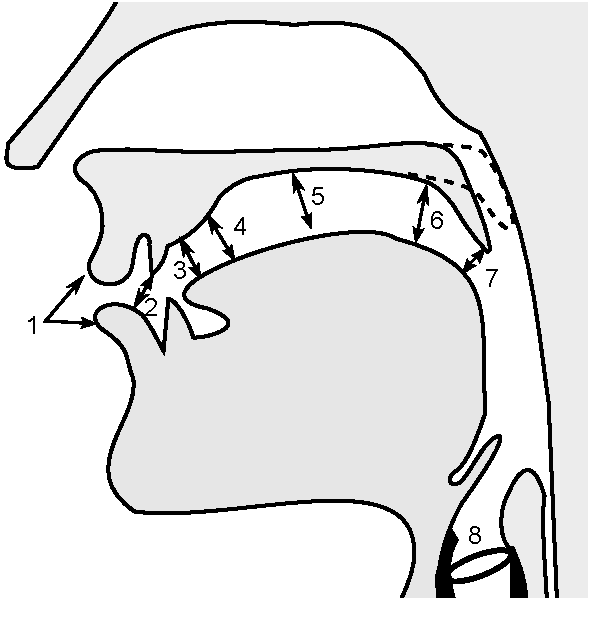
\includegraphics[width=.5\textwidth]{figures/PlaceOfArticulation5.pdf}
    \caption{Artikulationsorte im Deutschen: (1) bilabial, (2) labiodental, (3) alveolar, (4) postalveolar, (5) palatal, (6) velar, (7) uvular, (8) glottal. Das Zäpfchen kann angehoben werden (gestrichelte Linie). Quelle: Tavin, Wikimedia Commons über creative commons licence CC BY 3.0, adaptiert \url{https://commons.wikimedia.org/wiki/File:PlaceOfArticulation.svg}}
    \label{Abb:Artikulationsorte}
\end{figure}

Im Folgenden\is{bilabial} wird untersucht, welche Laute an den einzelnen Orten gebildet werden können. Die Laute zu Beginn der Wörter \textit{Bein}, \textit{Panne} und \textit{Mensch} werden mit beiden Lippen gebildet, was in der Abbildung als (1) dargestellt ist.  Im internationalen phonetischen Alphabet werden diese Laute mit \textipa{[b, p]} und \textipa{[m]} notiert. Diese Laute nennt man \textit{bilabiale} Laute (mit beiden Lippen gebildet).

 Die Wörter \textit{finden}\is{labiodental} und \textit{winden} beginnen mit Lauten, bei denen man die Unterlippe gegen die oberen Schneidezähne legt. Im IPA werden diese Laute \textipa{[f]} und \textipa{[v]} geschrieben. Laute, die mit der Unterlippe und den oberen Schneidezähnen gebildet werden, bezeichnet man als \textit{labiodentale} Laute (Artikulationsort (2) in der Abbildung).

Die Anlaute der Wörter \textit{Nase, leben, tanzen}\is{alveolar} werden mit der Zunge am Zahndamm gebildet (Artikulationsort (3) in der Abbildung). Diese Laute bezeichnet man als \textit{alveolare} Laute. Im IPA werden die Anlaute aus den Beispielwörtern mit \textipa{[n, l, t]} notiert. Im Deutschen gibt es sehr viele alveolare Laute.

Wenn\is{postalveolar} man den Laut \textipa{[s]} lang andauernd bildet und die Zungenspitze dabei ein bisschen zurückzieht, entsteht der Laut \textipa{[S]}, der Anlaut des Wortes \textit{Schule}. Dieser Laut wird hinter den Alveolen gebildet, also \textit{postalveolar} (Artikulationsort (4) in der Abbildung). 

Welche\is{ingressiv} Laute im hinteren Bereich des Mundes an den Artikulationsstellen (5), (6) und (7) gebildet werden, ist schwerer direkt wahrnehmbar. Eine Methode, um die Artikulationsstelle einiger Laute (der sogenannten Frikative, vgl. Abschnitt \ref{subsubsection:Frikative}) wahrnehmbar zu machen, ist \textit{ingressives Sprechen}. Dabei spricht man, während man einatmet. Da die Luft von außerhalb des Vokaltrakts kälter als die Körpertemperatur ist, fühlt sich die Artikulationsstelle kalt an. Wenn man \textipa{[s]} ingressiv produziert, wird es an den Alveolen kalt. Beim \textipa{[\c{c}]}, dem letzten Laut in \textit{ich}, wird es am harten Gaumen kalt. Bei \textipa{[\c{c}]} handelt es sich also um einen \textit{palatalen Laut}\is{palatal} (Artikulationsstelle (5) in der Abbildung). 

Der\is{velar} letzte Laut im Wort \textit{Buch}, \textipa{[x]}, ist ein velarer Laut, er wird am weichen Gaumen gebildet. Auch diese Artikulationsstelle (6) ist erfahrbar, wenn wir den Laut ausgedehnt ingressiv sprechen.

Für\is{uvular} die meisten deutschen Sprecherinnen und Sprecher gibt es perzeptiv keinen Unterschied zwischen dem <ch> in \textit{Buch} und \textit{Bach}. Sie klingen gleich. Nach \textipa{[a]} sprechen wir <ch> jedoch als \textipa{[\textchi]}, einen \textit{uvularen} Laut . Uvulare Laute werden am Zäpfchen gebildet. In der Abbildung entspricht das der Artikulationsstelle (7).

Zu\is{glottal} den \textit{glottalen} Lauten an Artikulationsstelle (8) gehört das \textipa{[h]}, der Anlaut von \textit{Haus}. Dieser Laut wird durch eine Verengung an den Stimmlippen produziert. Durch die Verengung wird die Luft aus der Lunge verwirbelt und erzeugt so das Rauschen, das für diesen Laut typisch ist. 

\subsection{Artikulationsarten}

An manchen Artikulationsorten werden sehr viele Laute gebildet, an den Alveolen etwa \textipa{[s, l, n, t]} und andere. Trotzdem klingen diese Laute sehr verschieden, was nicht nur auf Unterschiede in der Stimmhaftigkeit zurückzuführen ist. Die hauptsächliche Ursache für den unterschiedlichen Klang ist, dass die Laute auf unterschiedliche Arten gebildet werden.


\subsubsection{Plosive}
\label{subsection:Plosive}
\is{Plosiv}

Laute wie \textipa{[p, d, k]} werden gebildet, indem man im Vokaltrakt einen Verschluss produziert. Bei \textipa{[p]}wird der Verschluss an den Lippen produziert, bei \textipa{[d]} an den Alveolen und bei \textipa{[k]} im velaren Bereich. Da während des Verschlusses weiter Luft aus der Lunge Richtung Lippen strömt, erhöht sich der Luftdruck hinter der Verschlussstelle. Wenn der Verschluss gelöst wird, entsteht ein Verschlusslösungsgeräusch\is{burst} (\textit{burst}). Laute, die auf diese Art und Weise gebildet werden, nennt man \textit{Plosive} (vgl. \gqq{Explosion}).

Plosive kann man leicht daran erkennen, dass man sie nicht langanhaltend produzieren kann. Laute wie \textipa{[f], [s]} oder \textipa{[\c{c}]} können wir einige Sekunden lang aushalten, Plosive hingegen nicht, da sie aus Verschluss und Verschlusslösung bestehen und die Verschlusslösung punktuell ist.

Plosive können stimmhaft oder stimmlos sein. Als stimmhaft klassifizieren wir die Plosive \textipa{[b, d, g]}, auch wenn sie nur intervokalisch vollständig stimmhaft sind (vgl. Abschnitt~\ref{sec:Stimmhaftigkeit}). Stimmlos sind die Plosive \textipa{[p, t, k]} und der an der Glottis gebildete \textit{Knacklaut} \textipa{[P]}. 

Der Knacklaut\is{Laute!Knacklaut} ist ein Laut, der keine orthografische Repräsentation hat. Er tritt im Deutschen regelhaft auf. Der Knacklaut ist ein glottaler Plosiv. Bei seiner Bildung sind die Stimmlippen zunächst fest gegeneinander gepresst. Unter der Glottis wird durch die Luft, die aus der Lunge kommt, ein erhöhter Druck aufgebaut. Dieser Druck führt dazu, dass die Glottis aufgesprengt wird, wobei ein Verschlusslösungsgeräusch entsteht. Für die meisten Hörerinnen und Hörer ist das Verschlusslösungsgeräusch (das Knacken) weniger prominent als die Verschlussphase selbst, die sie als kleine Pause wahrnehmen.

Wir betrachten dazu die Wörter \textit{einander} und \textit{ein anderer}. Im \citet{DudenRechtschreibung2024} ist das Wort \textit{einander} mit folgender Silbifizierung angegeben: \uarc{\textit{ei}}\uarc{\textit{nan}}\uarc{\textit{der}}.\footnote{Wir verwenden zur Demonstration der Silbengrenzen hier zunächst die Silbenbögen, die häufig auch in der Grundschule genutzt werden.} Das erste \textipa{[n]} gehört also zur zweiten Silbe. Bei \textit{ein anderer} ist das anders, hier ist die erste Silbengrenze mit der Wortgrenze identisch: \uarc{\textit{ein}} \uarc{\textit{an}}\uarc{\textit{de}}\uarc{\textit{rer}}. Akustisch besteht der Unterschied an der ersten Silbengrenze darin, dass bei \textit{ein anderer} vor dem \textipa{[a]} der Knacklaut gesprochen wird und bei \textit{einander} nicht. Ohne Knacklaut wäre die Silbifizierung \uarc{\textit{ei}}\uarc{\textit{nan}}\uarc{\textit{de}}\uarc{\textit{rer}}.

Den Knacklaut hört man auch vielfach bei nichtsprachlichen Äußerungen, etwa wenn man einen schweren Gegenstand absetzt. Um solche Gegenstände anzuheben, versucht man, den Oberkörper zu stabilisieren. Dazu atmet man ein und verschließt die Lunge durch das Zusammenpressen der Stimmlippen.\footnote{Deshalb kann man beim Anheben eines schweren Möbelstücks kaum atmen.} Wenn man den schweren Gegenstand wieder absetzt, löst man den Verschluss an der Glottis. Dabei entsteht ein Geräusch, so wie man es auch am Anfang eines Stöhnens hört. Das ist der Knacklaut.

Auch viele Sportlerinnen und Sportler produzieren den Knacklaut, zum Beispiel beim Tennisspielen, Kugelstoßen, Diskuswerfen oder Speerwerfen. Auch hier wird zuerst der Oberkörper stabilisiert, indem die Glottis geschlossen wird. Wenn der Ball geschlagen wurde oder die Kugel gestoßen usw. öffnen die Sportlerinnen und Sportler die Stimmlippen. Dabei entsteht der Knacklaut.

Als Sprachlaut wird der Knacklaut in Mittel- und Norddeutschland laut \citet[14, 65f]{DudenAussprache2023} unter folgenden Bedingungen produziert (vgl. Abschnitt~\ref{sec:Epenthese}): 
\begin{itemize}
    \item zu Beginn eines Wortes, wenn das Wort sonst mit Vokal anfangen würde, also \zB bei \textit{Apfel} \textipa{[\textprimstress Pa\.*{\t{pf}}@l]}, \textit{Eis} \textipa{[P\t*{aI}s]}, \textit{anders} \textipa{[\textprimstress Pan.d5s]}, \textit{Ende} \textipa{[\textprimstress PEn.d@]}.
    \item  innerhalb des Wortes am Anfang von betonten Silben, wenn diese sonst mit Vokal beginnen würden, etwa bei bei \textit{überall} \textipa{[\textsecstress Py:.b5\textprimstress Pal]} vor dem \textipa{[a]}, \textit{enteignen} \textipa{[PEnt\textprimstress P\t*{aI}.gn@n]} (vor dem <ei>), \textit{geändert} \textipa{[g@\textprimstress PEn.d5t]}.
\end{itemize}

In Süddeutschland wird der Knacklaut von älteren Generationen seltener produziert, in Österreich und der Schweiz wird er sehr selten gebraucht \citep[66]{DudenAussprache2023}.

Eine sehr saliente\footnote{\textit{Salient} bedeutet, dass der Kontrast hervorstechend ist.} Verwendung des Knacklautes findet man bei \is{geschlechtergerecht} geschlechtergerechter Sprache. Wir vergleichen dazu das Wort \textit{Studentinnen} mit \textit{Student$^\ast$innen} (und den akustisch ähnlich realisierten Formen \textit{Student:innen, StudentInnen, Student\_innen}). Betrachten wir zunächst wieder die Silbifizierung:

\ea
\ea \label{ex:StudentInnen} 
\uarc{Stu} \uarc{den} \uarc{tin} \uarc{nen}
\ex \uarc{Stu} \uarc{dent} \uarc{$^\ast$in} \uarc{nen}
\z
\z

Während die dritte Silbe von \textit{Studentinnen} mit dem Konsonanten \textipa{[t]} anfängt, beginnt die dritte Silbe von \textit{Student$^\ast$innen} orthografisch gesehen mit einem Vokal. An der Stelle des Sternchens, also vor diesem Vokal, wird ein Knacklaut gesprochen. Nach der Regel, die wir oben angegeben haben, wird der Knacklaut nur am Wortanfang oder in betonten Silben eingesetzt. Viele Sprecherinnen und Sprecher betonen bei \textit{Student$^\ast$innen} tatsächlich die dritte Silbe,  wie in Beispiel (\ref{ex:StudentInnen_Transkription}) gezeigt, während sie die weibliche Form in Beispiel (\ref{ex:Studentinnen_Transkription}) auf der zweiten Silbe betonen:

\ea
\ea \label{ex:Studentinnen_Transkription} 
Studentinnen: \textipa{[Stu\textprimstress dEn.tI\.*n@n]}
\ex \label{ex:StudentInnen_Transkription} Student$^\ast$innen: \textipa{[Stu\textsecstress dEnt\textprimstress PI\.*n@n]}
\z
\z



\subsubsection{Frikative}\label{subsubsection:Frikative}
\is{Frikativ}
Frikative sind Laute, bei denen kein Verschluss, sondern eine Enge im Vokaltrakt gebildet wird. Ein Beispiel für einen Frikativ ist der Laut \textipa{[f]}. Bei diesem Laut wird zwischen Unterlippe und oberen Schneidezähnen eine Enge (sogenannte \textit{Konstriktion}\is{Konstriktion}) gebildet, durch die bei der Produktion des Lautes Luft fließt. Die Luft wird beim Passieren der Enge verwirbelt, sodass ein Rauschen entsteht. Dieser Vorgang ist vergleichbar mit der Turbulenzbildung in Flüssen, die Engen passieren.

Ob es tatsächlich zur Verwirbelung und damit zur Rauschbildung kommt, ist, wie \citet{Shadle85} zeigt, vom Verhältnis der Konstriktion zur Geschwindigkeit der Luft abhängig: Wenn man die Konstriktion sehr eng produziert (die Unterlippe also fast schon gegen die Zähne gepresst wird), kann die Fließgeschwindigkeit der Luft geringer sein, um Rauschen zu produzieren. Wenn die Konstriktion eher weit ist, muss die Geschwindigkeit der Luft höher sein, um Rauschen zu erzeugen. Ist weder das eine noch das andere gegeben (die Konstriktion ist weit und die Fließgeschwindigkeit niedrig), kann kein Rauschen erzeugt werden.

Eine\is{Sibilant} besondere Klasse innerhalb der Frikative bilden die \textit{Sibilanten} \textipa{[s, z, S]}, die in den Anlauten der Wörter \textit{Skelett} \textipa{[ske\textprimstress lEt]}, \textit{Sonne} \textipa{[\textprimstress zO\.*{n}@]}\footnote{Diese Aussprache empfiehlt das \citet[139]{DudenZweifelsfaelle2021}. Im Süddeutschen, der Schweiz und Österreich spricht man jedoch meist \textipa{[\textprimstress sO\.*{n}@]} \citep[74]{DudenAussprache2023}, siehe auch Stefan Kleiner: \textit{Atlas zur Aussprache des deutschen Gebrauchsstandards (AADG)}. \url{https://prowiki.ids-mannheim.de} (Zugriff: 28.08.2025) zum Stichwort \textit{s im Anlaut}.} und \textit{Schule} \textipa{[\textprimstress Su:.l@]} vorkommen. Ein weiterer Sibilant ist das \is{nativ} nichtnative\footnote{\textit{Nativ} bedeutet, dass diese Laute im nativen (nicht fremdsprachlichen) Wortschatz vorkommen. \textipa{[s]} kommt \zB im Erbwort \textit{messen} vor und ist deshalb nativ. Der Anlaut des Wortes \textit{Thinktank} \textipa{[\texttheta]} ist kein nativer Laut, denn er kommt nur in Fremdwörtern vor, genauso wie \textipa{[Z]}. Den Stamm \textit{nativ} findet man auch in \textit{native speaker, digital native}.}  \textipa{[Z]}, welches in  \textit{Genie} \textipa{[Ze\textprimstress ni:]} vorkommt. Sibilanten sind Laute, bei denen der Luftstrom zunächst -- wie bei allen Frikativen -- eine Konstriktion passiert, hinterher aber noch gegen ein Hindernis geleitet wird. Dieses Hindernis sind die Schneidezähne. \citet{Shadle1991} zeigt, dass an den Schneidezähnen eine weitere Verwirbelung der Luft erfolgt, sodass Sibilanten sich durch ein besonders intensives hochfrequentes Rauschen auszeichnen.\footnote{Am Telefon kann man \textipa{[s]} und \textipa{[f]} nicht immer gut unterscheiden. Wenn man ein Wort mit <s> buchstabiert, versteht der Kommunikationspartner häufig <f>. Das liegt daran, dass über das Telefon nur Frequenzen bis 3,4kHz übertragen werden. Die charakteristischen Eigenschaften des Lautes \textipa{[s]} (das hochfrequente Rauschen) liegen aber über 3,4kHz und werden deshalb nicht übertragen. In fließender Rede fällt das jedoch nicht auf, weil unser Gehirn die fehlenden Informationen ergänzt.}


\begin{Exkurs}{Warum klingen \textipa{[s]} und \textipa{[z]} bei Kindern manchmal gelispelt?}
\label{Exkursgelispeltess}

\noindent Die wichtige Rolle der Schneidezähne bei den Sibilanten wird deutlich, wenn man versucht, Sibilanten mit großem Abstand zwischen den Schneidezähnen zu produzieren (also mit tiefem Kiefer). Sprechen Sie dazu zunächst ein paarmal \textit{lalala} und versuchen Sie dann, bei \textipa{[l]} anzuhalten. Legen Sie dabei einen Finger an Ihr Kinn, um die Kieferposition zu kontrollieren. Versuchen Sie nun, zu einem \textipa{[s]} zu wechseln und dabei die Kieferposition unverändert zu lassen. Wenn Ihnen das gelingt, sollte das \textipa{[s]} weniger intensiv, möglicherweise \gqq{gelispelt} klingen. Das liegt daran, dass Sie den Luftstrom nun nicht mehr gegen die unteren Schneidezähne leiten können.

Möglicherweise bewegen Sie auch ganz automatisch den Kiefer nach oben. Dann klingt das \textipa{[s]} normal, eben weil der Luftstrom gegen die unteren Schneidezähne geleitet wird und dort weitere Turbulenzen entstehen.

Nun aber zur Ausgangsfrage: Warum klingen \textipa{[s]} und \textipa{[z]} bei Kindern, vor allem im Alter von 6--7 Jahren, manchmal gelispelt? Diesen Kindern fehlen häufig ein oder mehrere Schneidezähne, weil sie gerade ihr Milchgebiss verlieren. Dadurch muss der Luftstrom nicht, wie bei Menschen mit vollständigem Gebiss, ein zweites Hindernis passieren. Das führt (wie bei dem Experiment eben) zu einem weniger intensiven Rauschen. Wenn die Kinder vor dem Zahnverlust nicht gelispelt haben, werden sie die Laute aller Wahrscheinlichkeit nach unauffällig sprechen, sobald das Gebiss wieder vollständig ist.
\end{Exkurs}

\largerpage
Sobald Sprecher(innen) des Deutschen alphabetisiert sind,\is{Laute![s]} finden sie es oft schwierig, \textipa{[s]} und \textipa{[z]} zu unterscheiden. Das liegt unter anderem daran, dass die Schreibung wenig Aufschluss über die Lautung gibt. \textipa{[s]} kann als <s, ss> oder <ß> (\textit{mie\underline{s}, vermi\underline{ss}en, Fü\underline{ß}e}) geschrieben werden. \textipa{[z]} wird immer <s> geschrieben (\textit{We\underline{s}en}). Um den Unterschied zwischen den Lauten \textipa{[s]} und \textipa{[z]} zu verdeutlichen, benutzen wir eine Terminologie aus der Kinder-Logopädie (\zB \cite[45ff]{FoxBoyeretal2015}). \textipa{[s]} wird in der Kinder-Logopädie \gqq{Schlangenlaut} genannt, weil man mit diesem Laut das Zischen einer Schlange imitieren kann. Das stimmhafte \textipa{[z]} wird als \gqq{Bienenlaut} bezeichnet -- das Summen einer Biene wird imitiert.  

Viele Laute können in jeder Position vorkommen, das \textipa{[p]} zum Beispiel initial in \textit{Panne} \textipa{[\textprimstress pa\.*n@]}, medial in \textit{Happen} \textipa{[\textprimstress ha\.*p@n]}, alternativ \textipa{[\textprimstress ha\.*p\s{m}]}, und final in \textit{stopp} \textipa{[StOp]}. Das ist bei den beiden alveolaren Frikativen \textipa{[s]} und \textipa{[z]} nicht so. Im norddeutschen Standard kommt das \textipa{[s]} nur medial, \zB in \textit{Masse} \textipa{[\textprimstress ma\.*s@]} und \textit{Grüße} \textipa{[\textprimstress gKy:s@]} und final, \zB  in \textit{Bus} \textipa{[bUs]}, \textit{Bass} \textipa{[bas]} und \textit{Gruß} \textipa{[gKu:s]} vor. Initial ist es sehr eingeschränkt. Es kommt in Fremdwörtern wie \textit{Cent} \textipa{[sEnt]} und in Konsonantenverbindungen wie in \textit{Skandal} \textipa{[skan\textprimstress da:l]} vor. Ansonsten ist es auf den bairischen und schweizer Sprachraum begrenzt. Das Wort \textit{Sache} etwa wird im norddeutschen Standard \textipa{[\textprimstress za\.*x@]} gesprochen, im bairischen und schweizer Raum aber \textipa{[\textprimstress sa\.*x@]} \citep[74]{DudenAussprache2023}.

Das \textipa{[z]}\is{Laute![z]} ist ebenfalls nicht in jeder Position zu finden. Es kommt initial vor, etwa in \textit{Sand} \textipa{[zant]} oder \textit{sieben} \textipa{[\textprimstress zi:.b@n]}, alternativ \textipa{[\textprimstress zi:b\s{m}]}, aber es steht auch medial, etwa in \textit{Faser} \textipa{[\textprimstress fa:.z5]} oder \textit{lesen} \textipa{[\textprimstress le:z@n]}, alternativ \textipa{[\textprimstress le:z\s{n}]}. Aufgrund der Auslautverhärtung (vgl. Abschnitt~\ref{sec:Auslautverhaertung}) kommt \textipa{[z]} aber nicht final vor. Man spricht zwar \textit{Mäuse} \textipa{[\textprimstress m\t*{OI}.z@]}, aber \textit{Maus} \textipa{[m\t*{aU}s]}, nicht \textipa{[m\t*{aU}z]}.

Der\is{Laute!ch-Laute} palatale Frikativ \textipa{[\c{c}]}, der velare \textipa{[x]} und der uvulare \textipa{[X]} werden orthografisch alle als <ch> repräsentiert. Auch diese Laute kommen nur in bestimmten Umgebungen vor, der Laut  \textipa{[\c{c}]} etwa in den folgenden drei:
\begin{itemize}
    \item nach den sogenannten Vorderzungenvokalen \textipa{[i, I, y, Y, e, E, \o, \oe]} (vgl. Abschnitt~\ref{sec:Vokale}), \zB in \textit{Bücher} \textipa{[\textprimstress bY:.\c{c}5]} oder \textit{Becher} \textipa{[\textprimstress bE\.*{\c{c}}5]}
    \item nach Konsonanten, \zB in \textit{Milch} \textipa{[mIl\c{c}]}
    \item zu Beginn eines Morphems\footnote{Ein Morphem ist eine bedeutungstragende Einheit, auch: Wortbaustein (vgl. Abschnitt~\ref{section:Einheiten Wortbildung}, \pageref{section:Einheiten Wortbildung}, Definition~\ref{def:Morphem}.)} \zB in \textit{Häuschen} \textipa{[h\t*{OI}s.\c{c}@n]}.
\end{itemize} 

Der velare Frikativ \textipa{[x]} wird nach den Hinterzungenvokalen \textipa{[u, o]}, \zB in \textit{Buch} \textipa{[bu:x]} und \textit{hoch} \textipa{[ho:x]} gesprochen. Der uvulare Laut \textipa{[X]} wird nach \textipa{[a, U, O]} gesprochen: \textit{Dach} \textipa{[daX]}, \textit{Bucht} \textipa{[bUXt]}, \textit{Koch} \textipa{{kOX}} (vgl. Abschnitt~\ref{sec:Allophone}, \cite[202]{Pompino-Marschall2020}).

Die stimmhafte Variante des uvularen Frikativs \textipa{[X]} ist \textipa{[K]}. Dieser Laut kann initial im Wort \textit{Raum} \textipa{[K\t*{aU}m]} gesprochen werden. Laut \citet[52]{DudenAussprache2023} ist \textipa{[K]} die häufigste Art, den r-Laut zu sprechen und -- außer in Teilen der Schweiz -- überall gebräuchlich. Im Gegensatz zu den anderen beiden r-Varianten ist \textipa{[K]} nicht gerollt, sondern am Zäpfchen gerieben (vgl. Abschnitt~\ref{sec:Vibranten}).

Auch das \textipa{[h]}\is{Laute![h]} ist ein Frikativ. Es wird an der Glottis produziert. Die Engebildung erfolgt bei diesem Laut zwischen den Stimmlippen. Die Stimmlippen nähern sich dazu einander an, jedoch ohne dass die Glottis geschlossen wird.




\subsubsection{Nasale}\label{subsec:Nasale}

Die Wörter \textit{Nase} und \textit{Masse} beginnen mit einem Nasal.\is{Nasal} Bei Nasalen wird der Mund an einer Stelle verschlossen - bei \textipa{[m]} an den Lippen und bei \textipa{[n]} an den Alveolen. Das Velum wird gleichzeitig gesenkt, sodass die Luft nicht durch den Mund, sondern durch die Nase entweicht. 

Artikulatorisch gesehen sind Nasale den Plosiven sehr ähnlich, weil auch bei den Plosiven der Mund an einer Stelle verschlossen wird. Abbildung~\ref{fig:Plosiv_Nasal} zeigt auf der linken Seite einen Sagittalschnitt für \textipa{[p]} und auf der rechten für \textipa{[m]}. Der einzige Unterschied zwischen den beiden Konfigurationen ist das Velum, welches bei \textipa{[p]} gehoben ist und bei \textipa{[m]} gesenkt, sodass die Luft durch die Nase entweichen kann. Im Mundraum unterscheiden sich die Laute nicht.\is{Velum}

\begin{figure}
     \centering
     \begin{subfigure}[b]{0.4\textwidth}
         \centering
         
\includegraphics[width=\textwidth]{figures/Voiceless_bilabial_plosive.svg.png}
         \caption{Bilabialer Plosiv \textipa{[b]} oder \textipa{[p]}}
         \label{fig:bilabialer_Plosiv}
     \end{subfigure}
     \hfill
     \begin{subfigure}[b]{0.4\textwidth}
         \centering
         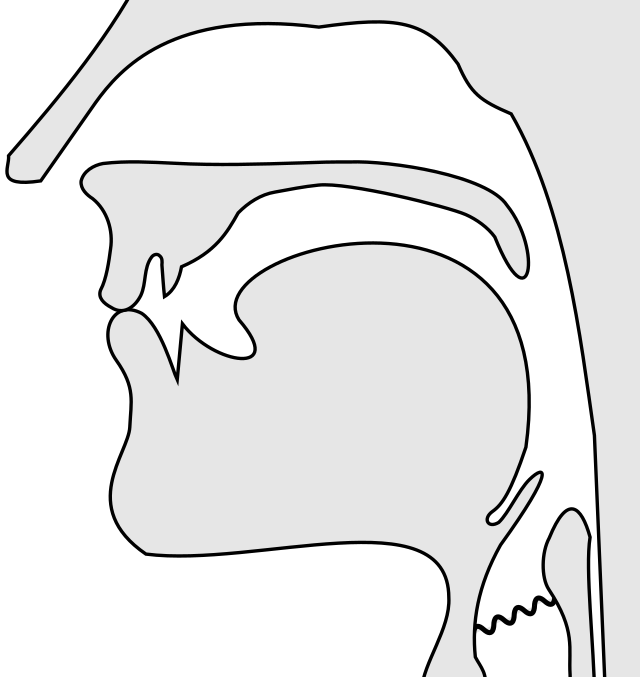
\includegraphics[width=\textwidth]{figures/Voiced_bilabial_nasal.svg.png}
         \caption{Bilabialer Nasal \textipa{[m]}}
         \label{fig:bilabialer_Nasal}
     \end{subfigure}
        \caption{Artikulatorische Konfigurationen der Plosive und Nasale. Quelle: Tavin, Wikimedia Commons über creative commons licence CC BY-SA 4.0, \url{https://commons.wikimedia.org/wiki/File:Voiceless\_bilabial\_plosive.svg}, \url{https://commons.wikimedia.org/wiki/File:Voiceless\_bilabial\_nasal.svg}}
        \label{fig:Plosiv_Nasal}
\end{figure}



Ob ein Laut ein Nasal ist, kann man feststellen, indem man die Nasalpassage verschließt (sich also die Nase zuhält). Wenn der Laut dann nicht mehr gebildet werden kann, handelt es sich um einen Nasal. Laute wie \textipa{[p, s, l]} können mit geschlossener Nase problemlos gebildet werden -- weil sie keine Nasale sind. Die Nasale \textipa{[m]} in \textit{Mensch} \textipa{[mEnS]}, \textipa{[n]} in \textit{nehmen} \textipa{[\textprimstress ne:.m@n]}, alternativ \textipa{[\textprimstress ne:.m\s{n}]} oder \textipa{[\textprimstress ne:.m:]}, und \textipa{[N]}, der letzte Laut in \textit{eng} \textipa{[PEN]}, sind jedoch mit geschlossener Nase nicht produzierbar.

Ein weiteres Indiz dafür, dass die Luft bei den Nasalen tatsächlich durch die Nase fließen muss, liefern Sprecherinnen und Sprecher, die erkältet sind. Wenn die Nase zugeschwollen ist, klingen die Nasale perturbiert.

Nasale sind eher leise Laute. Das liegt einerseits daran, dass der Schall in der Nasenhöhle gedämpft wird. Andererseits enthält das Nasalspektrum sogenannte \textit{Antiformanten}\is{Antiformant}. Wenn die Luft bei der Produktion von Vokalen von der Glottis bis zu den Lippen fließt, werden abhängig von der Zungen- und Lippenposition bestimmte Frequenzbereiche des Schalls verstärkt. Diese Bereiche nennt man Resonanzen oder \textit{Formanten}\is{Formant}. Wenn der Schall von der Glottis bis zu den Nasenlöchern fließt, entstehen ebenfalls Formanten. Die verschlossene Mundhöhle, die als Seitenarm der Passage von der Glottis bis zu den Nasenlöchern fungiert, schwächt einzelne Frequenzbereiche allerdings ab, anstatt sie zu verstärken. Dadurch entstehen Antiformanten, das sind Frequenzbereiche mit niedriger Amplitude \citep[Kap.9]{Johnson:2003}. 

Die Antiformanten machen das Nasalspektrum wenig charakteristisch. Deshalb sind Nasale schwer voneinander zu unterscheiden. Besonders die Laute \textipa{[m]} und \textipa{[n]} unterscheiden die meisten Hörerinnen und Hörer nicht auditiv, sondern visuell: Sie schauen auf die Lippen des Sprechers oder der Sprecherin und können so feststellen, ob es sich um einen bilabialen oder alveolaren Nasal handelt. Sehbehinderte Hörerinnen und Hörer finden es häufig schwierig, diese beiden Laute ohne Kontext zu unterscheiden. Auch beim Schriftspracherwerb kann es deshalb zu Verwechslungen von <m> und <n> kommen.

Aber auch mit durchschnittlichem Sehvermögen lernen wir die beiden Laute, wenn sie in weniger prominenten Positionen stehen (etwa als Flexionsendung), häufig erst über die Schrift zu unterscheiden. Davon zeugen die Äußerungen von Kindern zu Beginn des Schriftspracherwerbs in (\ref{ex:nstattm1}) und (\ref{ex:nstattm2}). Die entscheidenden Stellen sind durch Großbuchstaben markiert.

\ea
\ea \label{ex:nstattm1} Schriftliche Äußerung:\\ <aber du must noch ein bischen merr an deineN stiel arbeiten> (Schülerin der 2. Klasse, 8 Jahre alt\footnote{Karlsruhe Childen's Text Corpus, \citet{Lavalleyetal2015}})
\ex \label{ex:nstattm2} Mündliche Äußerung:\\ \textit{Ipalat, Ipalat, tut deN Hals gut, Ipalat} (Schüler der 1. Klasse, 6 Jahre alt, Hörbeleg auf einem Schulhof)
\z
\z
Diese Fehler basieren in der Regel nicht auf ungenügenden Flexionskenntnissen. Kinder in diesem Alter produzieren nämlich den Dativ femininer Substantive, wo keine Opposition zwischen \textipa{[n]} und \textipa{[m]} besteht, in der Regel korrekt: \textit{an deinER Geschichte arbeiten} (nicht \textit{deine}), \textit{tut DER Nase gut} (nicht \textit{die}).

Die\is{Vokal!nasal} nasalen Konsonanten dürfen nicht mit den nasalen Vokalen verwechselt werden. Der Unterschied zwischen nasalen Konsonanten und nasalen Vokalen besteht darin, dass es bei den Konsonanten einen vollständigen oralen Verschluss gibt. Bei nasalen Vokalen hingegen fließt die Luft gleichzeitig durch Mund und Nase \citep[163--166]{Johnson:2003}.

Nasale Vokale produzieren im deutschen Sprachraum nur wenige Sprecherinnen und Sprecher überhaupt, und dann nur in französischen Lehnwörtern wie etwa \textit{Restaurant} \textipa{[KEs.to\textprimstress r\~{\textscripta}]} oder \textit{Balkon} \textipa{[bal\textprimstress k\~{O}]}. Die meisten Sprecher(innen) neigen eher dazu, nasalierte Vokale in Fremdwörtern einzudeutschen: In Nord- und Mitteldeutschland \zB indem ein velarer nasaler Konsonant gesprochen wird, etwa \textit{Balkon} \textipa{[bal\textprimstress kON]}, \textit{Restaurant} \textipa{[KEs.to\textprimstress KaN]} oder \textipa{[KEs.to\textprimstress KON]}, \textit{Ragout fin} \textipa{[Ka.gu\textprimstress fEN]} \citep[35, 69]{DudenAussprache2023}. In Österreich und der Schweiz wird statt des \textipa{[N]} am Ende eher \textipa{[n]} gespochen, bei \textit{Balkon}  also \textipa{[bal\textprimstress ko:n]}.\footnote{Stephan Elspaß \& Robert Möller: \textit{Atlas zur deutschen Alltagssprache (AdA)}. \url{https://www.atlas-alltagssprache.de} (Zugriff am 28.08. 2025), Stefan Kleiner: \textit{Atlas zur Aussprache des deutschen Gebrauchsstandards (AADG)}. \url{https://prowiki.ids-mannheim.de} (Zugriff am 28.08.2025)}


\subsubsection{Vibranten}
\label{sec:Vibranten}
\is{Vibrant} Vibranten werden auch als gerollte Laute bezeichnet. Ein typisches Beispiel ist das gerollte Zungenspitzen-r. Die Produktion von Vibranten ist in gewisser Weise vergleichbar mit der des Stimmtons (vgl. Abschnitt~\ref{sec:Stimmhaftigkeit}): Es wird ein Verschluss gebildet und der Luftdruck hinter dem Verschluss steigt so lange, bis der Verschluss aufgesprengt wird. Beim Aufsprengen fließt die Luft durch die Artikulationsstelle. Durch die Stömung nimmt der Luftdruck an der Artikulationsstelle ab und es erfolgt ein Sog in einem Winkel von 90 Grad zur Strömung (\isi{Bernoulli-Effekt}). Dadurch  entsteht sofort ein weiterer Verschluss. Bei einem in fließender Rede produzierten Vibranten kommt es meist zu 2--3 Verschlusslösungen.

Im Unterschied zur Produktion von Stimmton, die im Kehlkopf an der Glottis stattfindet, werden Vibranten in der Mundhöhle produziert. Außerdem erfolgt das Öffnen und Schließen mit einer viel geringeren Frequenz als beim Stimmton. Wir können bei Vibranten deshalb akustisch einzelne Verschließ- und Öffnungsereignisse wahrnehmen, während wir Stimmton nicht als eine Abfolge von Öffnen und Schließen, sondern als Ton wahrnehmen.

Um einen Vibranten zu produzieren, benötigt man einen Artikulator, der sich sehr schnell bewegen kann. Dafür kommen nur die Lippen, die Zungespitze und die Uvula in Frage. Mit den Lippen können wir, wie in Abschnitt~\ref{sec:Vokaltrakt} angesprochen, einen bilabialen Vibranten produzieren. Dieser Laut wird im Deutschen allerdings nur in nonverbaler Funktion verwendet.

Viele Sprecherinnen und Sprecher produzieren den r-Laut als Vibranten. Dabei gibt es zwei Möglichkeiten, das Zungenspitzen-r und das gerollte Zäpfchen-r. Das Zungenspitzen-r \textipa{[r]} produziert man, indem man die Zungenspitze gegen die Alveolen legt -- wie für ein \textipa{[t]} -- und dann Luft durchbläst. Dabei muss die Zungenspitze aber so entspannt sein, dass sie anfängt zu vibrieren (ansonsten entsteht ein \textipa{[s]}). Diese Realisation findet sich vor allem im süddeutschen und österreichischen Raum.

Das gerollte Zäpfchen-r \textipa{[\;R]} produziert man, indem man den Zungenrücken an die Uvula (das Zäpfchen) legt. Dann bläst man Luft durch diesen Verschluss, sodass die Uvula zu vibrieren beginnt. Das gerollte Zäpfchen-r kommt vor allem vor, wenn etwas besonders hervorgehoben werden soll, \zB in kontrastierenden Kontexten: \textit{Ich habe nicht Leiter gesagt, sondern Rrreiter.}

\subsubsection{Approximanten}

\is{Approximant}Approximanten werden auch \is{Approximant!Halbvokal} \textit{Halbvokale} genannt. Das liegt daran, dass sie artikulatorisch und akustisch den Vokalen sehr nahe sind. Im Deutschen gibt es nur einen Approximanten, das \textipa{[j]}, wie in \textit{jung} \textipa{[jUN]}. Der Begriff Approximant ist darauf zurückzuführen, dass ein Artikulator sich an eine Artikulationsstelle annähert (lat. \textit{approximare} 'sich annähern'), ohne jedoch eine geräuschbildende Enge zu produzieren.

Approximanten\is{Frikativ} werden also durch eine Verengung im Vokaltrakt produziert; allerdings ist die Verengung nicht so eng, dass es zu Turbulenzen kommt. Im Unterschied zu den Frikativen, die auch durch eine Engebildung verursacht werden, wird die Luft bei den Approximanten nicht verwirbelt und es entsteht kein intensives Rauschen. Den Luftstrom bei den Approximanten können wir uns vorstellen wie einen Fluss, der an einer Stelle etwas eingeengt wird. Das Wasser fließt an der Stelle etwas schneller, aber es entstehen keine Strudel \is{laminarer Luftstrom}(laminarer Luftstrom). Der Luftstrom bei einem Frikativ ist eher vergleichbar mit einem Fluss, der stark eingeengt wird, wodurch es zur Strudelbildung kommt \is{turbulenter Luftstrom}(turbulenter Luftstrom). 

Wir können den Unterschied zwischen Frikativen und Approximanten gut nachvollziehen, indem wir die Laute \textipa{[j]}, wie im Anlaut von \textit{jeder}, und \textipa{[\c{c}]}, wie im Auslaut von \textit{ich}, vergleichen. Wenn wir eine Sequenz wie \textipa{[\c{c}j\c{c}j]} sprechen, ist der Hauptunterschied der Stimmton, den wir für \textipa{[j]} brauchen, für den Frikativ jedoch nicht. Um das Rauschen für den Frikativ zu produzieren, müssen Sprecherinnen und Sprecher entweder die Konstriktion\is{Konstriktion} etwas verengen (die Zunge geht nach oben) oder die Fließgeschwindigkeit erhöhen. Letzteres erreicht man, indem man Druck auf die Lunge ausübt \citep[Abschnitt 1.2]{Pompino-Marschall2020}. Dass man das tut, merkt man daran, dass man für \textipa{[\c{c}]} die Bauchmuskeln stärker anspannt.

Bei \textipa{[j]}\is{Vokal} erfolgt die Verengung im palatalen Bereich. In Abschnitt~\ref{sec:KonsonantenundVokale} wurde gezeigt, dass das \textipa{[j]} sich artikulatorisch kaum vom Vokal \textipa{[i]} unterscheidet. Man zählt den Approximanten trotzdem nicht zu den Vokalen, weil er nur im Onset einer Silbe stehen kann (also vor dem Vokal) und den Vokal nicht ersetzen kann (vgl. Abschnitt~\ref{sec:KonsonantenundVokale}). Es gibt also Silben, die mit \textipa{[j]} beginnen: \textit{Jugend} \textipa{[\textprimstress ju:.g@nt]}, \textit{Joch} \textipa{[jOX]}, \textit{Koje} \textipa{[\textprimstress ko:.j@]}. Außerdem kann das \textipa{[j]} -- vor allem im nichtnativen\is{nativ} Wortschatz -- auch einem Konsonanten folgen, \zB in \textit{tja, Bjarne, Kjelt},\footnote{Wenn der vorangehende Laut stimmlos ist, überträgt sich dieses Merkmal auf das \textipa{[j]}, sodass der Laut entstimmt wird und damit dem \textipa{[\c{c}]} sehr ähnlich wird.} aber es kann ohne Vokal keine Silbe bilden. Im Deutschen kann \textipa{[j]} nicht in der Koda einer Silbe stehen.

\subsubsection{Laterale}
\is{Lateral}
\largerpage
Die Engebildung bei Frikativen und Approximanten erfolgt zentral, also in der Mitte des Vokaltrakts. Wir können das für uns erfahrbar machen, indem wir \is{ingressiv}ingressiv sprechen, also sprechen, während wir einatmen (vgl. Abschnitt~\ref{sec:Artikulationsorte}). Wenn man \textipa{[\c{c}]} ingressiv spricht, merkt man, dass es an der Artikulationsstelle im palatalen Bereich in der Mitte des Gaumens kalt wird. 

Laterale\footnote{Singular: \textit{der Lateral}, Plural: \textit{die Laterale}} sind Laute mit \textit{seitlicher Engebildung} \citep[183]{Pompino-Marschall2020}. Der einzige Lateral im Deutschen ist das \textipa{[l]}. Bei diesem Laut liegt die Zunge an der linken oder rechten Seite des Gaumens an. Auf der anderen Seite des Gaumens fließt die Luft entlang. Wenn man \textipa{[l]} ingressiv spricht, sollte man -- wenn die Artikulationsposition wirklich so ist wie beim egressiven Sprechen -- spüren, dass es auf einer Wangeninnenseite kälter wird als auf der anderen.

In \is{Approximant!lateral}einigen Lehrwerken werden die Laterale zu den Approximanten gezählt und bilden dort die Untergruppe der lateralen Approximanten. Die Laterale unterscheiden sich von den zentralen Approximanten\is{Approximant!zentral} tatsächlich nur darin, dass die Enge bei den Lateralen seitlich ist. Das Verhalten des Luftstroms (keine Turbulenzen beim Passieren einer Enge) ist bei den beiden Lautklassen gleich.


\subsubsection{Affrikaten}\label{sec:Affrikaten}
\is{Affrikate}
Zu den Affrikaten\footnote{Singular: \textit{die Affrikate}, Plural: \textit{die Affrikaten}} zählen im Deutschen \textipa{[\t{pf}]}, wie in \textit{Apfel} \textipa{[\textprimstress Pa\.*{\t{pf}}@l]}, \textipa{[\t{ts}]}, wie in \textit{Katze} \textipa{[\textprimstress ka\.*{\t{ts}}@]} und \textipa{[\t{tS}]} wie in \textit{Gletscher} \textipa{[\textprimstress glE\.*{\t{tS}}5]}. Affrikaten sind \textit{homorgane\is{homorgan} Plosiv-Frikativ-Verbindungen}. \is{homorgan}Homorgan bedeutet, dass beide Laute, der Plosiv und der Frikativ, an etwa derselben Stelle gebildet werden.  Im nichtnativen Wortschatz gibt es zusätzlich zu den drei genannten Affrikaten\is{Laute![d͡ʒ]} noch das \textipa{[\t{dZ}]}, das etwa in \textit{Gin} \textipa{[\t{dZ}In]} vorkommt.\footnote{Die nichtnative Affrikate\textipa{[\t{dZ}]} ist nicht gleichzusetzen mit dem ebenfalls nichtnativen Frikativ \textipa{[Z]}. Die Affrikate spricht man in \textit{Job} \textipa{[\t{dZ}Ob]} (wenn man es englisch ohne Auslautverhärtung spricht), \textit{Dschungel} \textipa{[\textprimstress \t{dZ}U\.*N@l]}, \textit{Gender} \textipa{[\t{dZ}En.d5]}. Den Frikativ spricht man in \textit{Journal} \textipa{[ZUK\textprimstress na:l]} oder \textit{Gelée} \textipa{[Ze\textprimstress le:]}.}


Für den Schriftspracherwerb relevant sind die Affrikaten aus verschiedenen Gründen. Die Affrikate \textipa{[\t{pf}]} wird im Onset einer Silbe in nichtstandardsprachlichen Varianten Mittel- und Norddeutschlands häufig auf den Frikativ \textipa{[f]} reduziert \citep[693]{DudenAussprache2023}, was zu kindlichen Schreibungen wie <feat> für \textit{Pferd} führt.

Die Affrikate \textipa{[\t{ts}]} wird abhängig von der Position innerhalb der Silbe unterschiedlich geschrieben. Im Onset einer Silbe schreibt man sie <z>, wie in \textit{Zeit} \textipa{[\t{ts}\t*{aI}t]} oder \textit{Zentrum} \textipa{[\textprimstress \t{ts}En.tKUm]}. Zwischen Vokalen schreibt man sie <tz> wie in \textit{Katze} \textipa{[\textprimstress ka\.*{\t{ts}}@]} oder \textit{hetzen} \textipa{[\textprimstress hE\.*{\t{ts}}@n]}. Nach Konsonanten schreibt man die Affrikate <z>, wie in \textit{Holz} \textipa{[hOl\t{ts}]}, \textit{März} \textipa{[mE5\t{ts}]} oder \textit{Prinz} \textipa{[pKIn\t{ts}]} (vgl. Abschnitt~\ref{subsubsubsec:spezSG}).

\newpage
\begin{Exkurs}{Warum betrachtet man Affrikaten nicht einfach als Abfolgen von Plosiv und Frikativ, sondern als eigenständige Segmente? }
\label{Exkurs:Affrikaten}

\noindent Ein Grund dafür, dass Affrikaten als \textit{ein} Segment angesehen werden, ist, dass zumindest zwei der drei nativen deutschen Affrikaten aus einem einzigen Segment entstanden sind. Während der Entwicklung des Althochdeutschen aus dem Germanischen kam es zu einem Lautwandel, der als 2. \isi{Lautverschiebung} bezeichnet wird \citep[185--187]{Schmidt1996}. Dabei wandelten sich die Plosive \textipa{[p, t]} und \textipa{[k]} in bestimmten Kontexten zu den homorganen\is{homorgan} Frikativen \textipa{[f, s]} und \textipa{[x]} oder \textipa{[X]} und in anderen Kontexten zu den Affrikaten \textipa{[\t{pf}, \t{ts}]} und in vielen Schweizer Dialekten auch \textipa{[\t{kx}]}. 

Wir können heute noch Folgen dieses Lautwandels erkennen, wenn wir Wörter aus einer germanischen Sprache, die diesen Lautwandel nicht mitgemacht hat, \zB Englisch, mit diachron verwandten Wörtern des Deutschen vergleichen. In Tabelle~\ref{tab:Lautverschiebung} sind einige Beispiele zu sehen. Das englische Wort \textit{pepper} enthält zweimal den Laut \textipa{[p]}. In der deutschen Entsprechung \textit{Pfeffer} stehen an den entsprechenden Stellen die Affrikate \textipa{[\t{pf}]} und der Frikativ \textipa{[f]}. Ähnliche Beispiele findet man auch für die Plosive {[t]} (\textit{cat} -- \textit{Katze}, \textit{water} -- \textit{Wasser}) und \textipa{[k]} (\textit{make} -- \textit{machen}).

\begin{table}
    \centering
        \caption{\label{tab:Lautverschiebung} Vergleich von englischen Wörtern (ohne Lautverschiebung) und etymologisch verwandten deutschen Wörtern (mit Lautverschiebung)}
    \begin{tabular}{lll}\lsptoprule
        Englisch & Deutsch & Lautwandel\\\midrule
        \textit{\underline{p}epper} & \textit{\underline{Pf}effer} & Plosiv \textipa{[p]} zu Affrikate \textipa{[\t{pf}]}\\
        \textit{pe\underline{pp}er} & \textit{Pfe\underline{ff}er}& Plosiv \textipa{[p]} zu Frikativ \textipa{[f]}\\
        \textit{ca\underline{t}} & \textit{Ka\underline{tz}e} & Plosiv \textipa{[t]} zu Affrikate \textipa{[\t{ts}]}\\
        \textit{wa\underline{t}er} & \textit{Wa\underline{ss}er} & Plosiv \textipa{[t]} zu Frikativ \textipa{[s]}\\
        \textit{ma\underline{k}e} & \textit{ma\underline{ch}en} & Plosiv \textipa{[k]} zu Frikativ \textipa{[X]}    \\\lspbottomrule
    \end{tabular}
\end{table}

In den niederdeutschen Dialekten gibt es die Affrikaten nicht, weil die Lautverschiebung nur im Mittel- und Oberdeutschen stattgefunden hat. Das zeigt sich in Produktionen wie \textipa{[Pa\.*p@l]} für \textit{Apfel}, \textipa{[kat]} für \textit{Katze}. 

Dadurch, dass die Affrikaten ursprünglich mal ein einziger Laut waren, kommen sie auch heute noch in Kontexten vor, in denen eigentlich nur einzelne Segmente auftreten können. Zum Beispiel kommen \citet[67--68]{Hall2000} zufolge im Deutschen in der Koda einer Silbe nur dann zwei Obstruenten\footnote{Obstruenten sind Plosive und Frikative (vgl. Abschnitt~\ref{sec:ObstSon}).} vor, wenn einer dieser Laute \is{koronal}koronal\footnote{\textit{Koronal} bedeutet, dass der Laut mit der Zungenspitze gebildet wird.} ist. Es gibt also Verbindungen wie \textipa{[kt]} wie in \textit{Akt}, \textipa{[st]} wie in \textit{Ast} oder \textipa{[ks]} wie in \textit{Fuchs}, aber keine Verbindungen wie \textipa{[px]} oder \textipa{[k\c{c}]}, wo keiner der Laute koronal ist. Die einzige Ausnahme ist die Affrikate \textipa{[\t{pf}]}, wie in \textit{Kopf}.

\end{Exkurs}


\subsection{Obstruenten und Sonoranten}
\label{sec:ObstSon}

Einige der oben besprochenen Lautklassen sind sich ähnlicher als andere. Beispielsweise gibt es Lautklassen, die Paare von stimmhaften und stimmlosen Lauten enthalten, \zB \textipa{[p]} und \textipa{[b]}, \textipa{[s]} und \textipa{[z]}, \textipa{[\t{tS}]} und \textipa{[\t{dZ}]}. Diese Paarigkeit betrifft Plosive, Frikative und Affrikaten. In den anderen Lautklassen gibt es nur stimmhafte Laute (Nasale, Vibranten, Approximanten und Laterale). Plosive, Frikative und Affrikaten sind außerdem immer mit starker Geräuschbildung  verbunden, die anderen Lautklassen nicht. Es ist deshalb sinnvoll, zwei Oberklassen zu bilden (vgl. Abbildung~\ref{Abb:Konsonantenklassen}). Die erste Klasse, bestehend aus Plosiven, Frikativen und Affrikaten, nennen wir \textit{Obstruenten}\is{Obstruent} (vgl. engl. \textit{to obstruct} \glq behindern\grq). Die zweite Klasse, bestehend aus Nasalen, Vibranten, Approximanten und Lateralen, nennen wir  \textit{Sonoranten}\is{Sonorant} (vgl. \textit{sonor}, \glq klangvoll\grq). In einigen Lehrwerken werden auch die Vokale zu den Sonoranten gezählt, weil sie ebenfalls stimmhaft sind und ohne Geräuschbildung auskommen.


\begin{figure}
\small
    \begin{forest}
    for tree={s sep-=.25ex}
    [Konsonanten
      [Obstruenten
        [Plosive [\textipa{[p]}]]
        [Frikative [\textipa{[z]}]]
        [Affrikaten [\textipa{[\t{ts}]}]]
      ]
      [Sonoranten
        [Nasale [\textipa{[n]}]]
        [Approximanten [\textipa{[j]}]]
        [Vibranten [\textipa{[r]}]]
        [Laterale [\textipa{[l]}]]
      ]
    ]
    \end{forest}
    \caption{Konsonantenklassen mit je einem Beispiel}
    \label{Abb:Konsonantenklassen}
\end{figure}

In Kapitel~\ref{kap:Phonologie} wird gezeigt, dass die Unterscheidung zwischen Sonoranten und Obstruenten auch sinnvoll ist, um die Abfolge der Segmente in der Silbe zu erklären. Die Obstruenten stehen in der Silbe nämlich immer ganz außen und die Sonoranten näher am Nukleus. So gibt es Silben wie \textit{klingt} \textipa{[klINt]}, wo die Ob\-stru\-enten 
\textipa{[k]} und \textipa{[t]} außen und die Sonoranten \textipa{[l]} und \textipa{[N]} um den Vokal herum stehen. Aber es gibt keine Silben wie *\textipa{[lka:tN]}, wo die Sonoranten außen um die Obstruenten herum stehen.

Außerdem ist die Unterscheidung zwischen Sonoranten und Obstruenten für orthografische Phänomene sinnvoll (vgl. Abschnitt~\ref{AbschnittDehnungsh}). So steht ein Dehnungs-\textit{h} in der Regel nur vor Sonoranten, wie in \textit{Ruhm, mehr, Bühne, kühl}.


\section{Vokale}\label{sec:Vokale}
\is{Vokal}
In Abschnitt~\ref{sec:Vokaltrakt} wurde eine MRT-Aufnahme des Vokaltrakts gezeigt. Diese Abbildung ist ganz links in Abbildung~\ref{fig:dreiVokale} noch einmal zu sehen. Die drei Darstellungen zeigen einen Sprecher, der unterschiedliche Vokale produziert. Ganz links ist die Vokaltraktkonfiguration für den Vokal \textipa{[a]} dargestellt. In der Mitte sieht man die Konfiguration für \textipa{[i]} und ganz rechts die Konfiguration für \textipa{[u]}.

\begin{figure}
     \centering
     \begin{subfigure}[b]{0.28\textwidth}
         \centering
         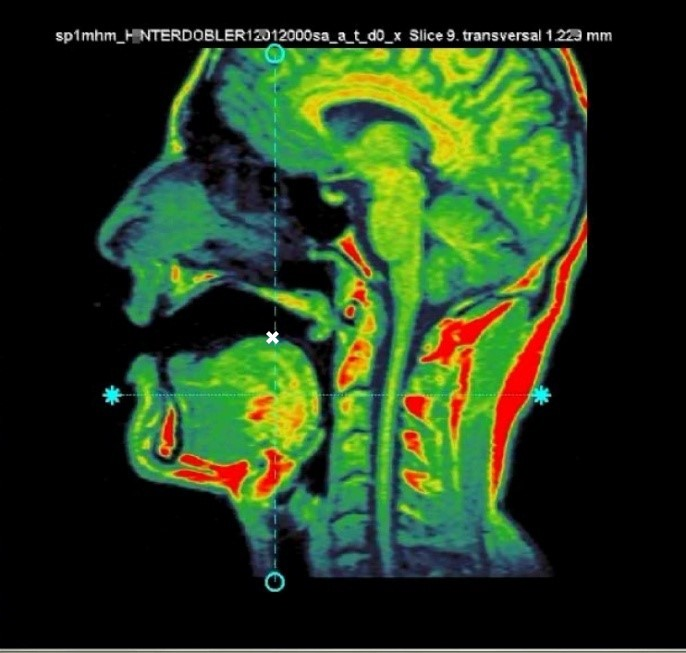
\includegraphics[width=\textwidth]{figures/mrt_a_Kreuz.jpg}
         \caption{[a]}
         \label{fig:Vokaltrakt_a}
     \end{subfigure}
     \hfill
     \begin{subfigure}[b]{0.3\textwidth}
         \centering
         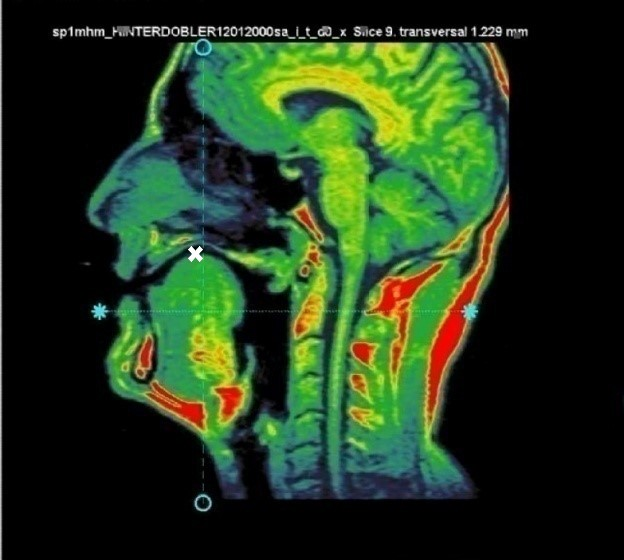
\includegraphics[width=\textwidth]{figures/mrt_i_Kreuz.jpg}
         \caption{[i]}
         \label{fig:Vokaltrakt_i}
     \end{subfigure}
     \hfill
     \begin{subfigure}[b]{0.32\textwidth}
         \centering
         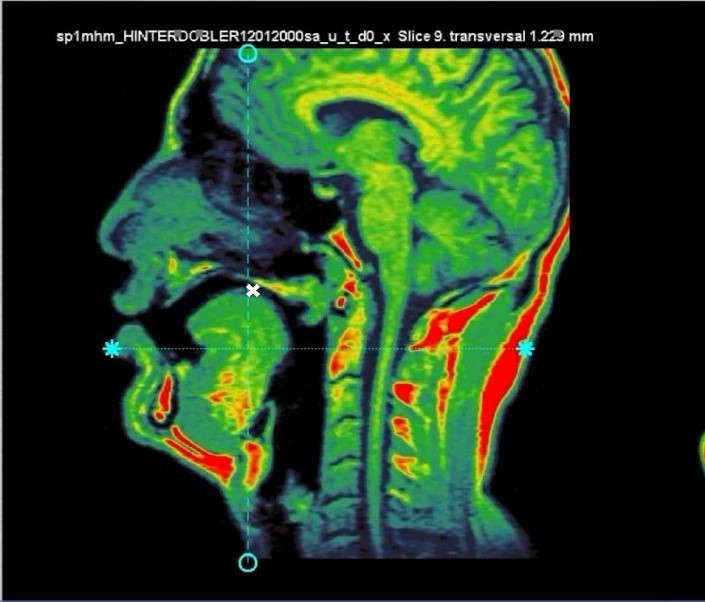
\includegraphics[width=\textwidth]{figures/mrt_u_Kreuz.jpg}
         \caption{[u]}
         \label{fig:Vokaltrakt_u}
     \end{subfigure}
        \caption{Vokaltraktkonfigurationen bei unterschiedlichen Vokalen (MRT-Aufnahmen, Quelle: Phil Hoole, Institut für Phonetik und Sprachverarbeitung, Ludwig-Maximilians-Universität München). Die weißen Kreuze wurden später hinzugefügt und markieren jeweils den höchsten Punkt des Zungenrückens.}
        \label{fig:dreiVokale}
\end{figure}

Man kann erkennen, dass die Zunge bei jedem Vokal eine andere Form annimmt. Bei \textipa{[a]} liegt sie relativ flach im Mund, bei \textipa{[i]} bildet sie im palatalen Bereich eine Verengung und bei \textipa{[u]} im velaren Bereich. Diese Unterschiede werden in der Phonetik als Unterschiede in der \is{Zungenhöhe}Zungenhöhe und der \is{Zungenlage}Zungenlage beschrieben. Der Referenzpunkt bei der Ermittlung der Zungenhöhe und Zungenlage ist der \textit{höchste Punkt des Zungenrückens}\is{Zungenrücken}, der als weißes Kreuz in den Abbildungen markiert ist. 

Die \is{Zungenhöhe}Zungenhöhe von \textipa{[a]} ist, verglichen mit den anderen beiden Lauten, \textit{tief}: Die Zunge liegt flach im Mund und das weiße Kreuz ist deutlich tiefer als bei \textipa{[i]} und \textipa{[u]}. Die Zungenhöhe von \textipa{[i]} und \textipa{[u]} ist, verglichen mit \textipa{[a]}, \textit{hoch}. Die \is{Zungenlage}Zungenlage von \textipa{[i]} ist \textit{vorn} (Vorderzungenvokal), denn das weiße Kreuz ist, verglichen mit \textipa{[u]}, relativ weit vorne. Die Zungenlage von \textipa{[u]} ist \textit{hinten} (Hinterzungenvokal). \textipa{[a]} ist im Deutschen von der Zungenlage her ein zentraler Vokal, die Zungenlage variiert abhängig von Kontext und Sprecher(in) sehr stark um die Mitte (\cite[14]{Becker1998}, \cite[225]{PaetzoldSimpson1997}, \cite[57]{Brunner2009}).

\subsection{Zungenhöhe und Zungenlage}

Zungenhöhe und Zungenlage eines Lautes können im \textit{Vokalviereck}\is{Vokalviereck} (auch: \textit{Vokaltrapez, Vokaldreieck}) dargestellt werden (vgl. Abbildung~\ref{fig:Vokalviereck}). Das Vokalviereck bezieht sich auf die Mittsagittale, also die Ebene, die den Kopf in eine gleich große rechte und linke Hälfte teilt. Auf dieser Ebene gibt das Vokalviereck an, ob Vokale im Vergleich zu anderen Vokalen weiter vorn, weiter hinten, weiter oben oder weiter unten gebildet werden.

Da man nicht die gesamte Kontur der Zunge auf einen Punkt reduzieren kann, bezieht sich die Darstellung auf den höchsten Punkt des Zungenrückens bei der Produktion des jeweiligen Vokals. Die weißen Kreuze in Abbildung~\ref{fig:dreiVokale} sind also die Referenzpunkte, die im Vokalviereck dargestellt werden.

\begin{figure}
    \centering
    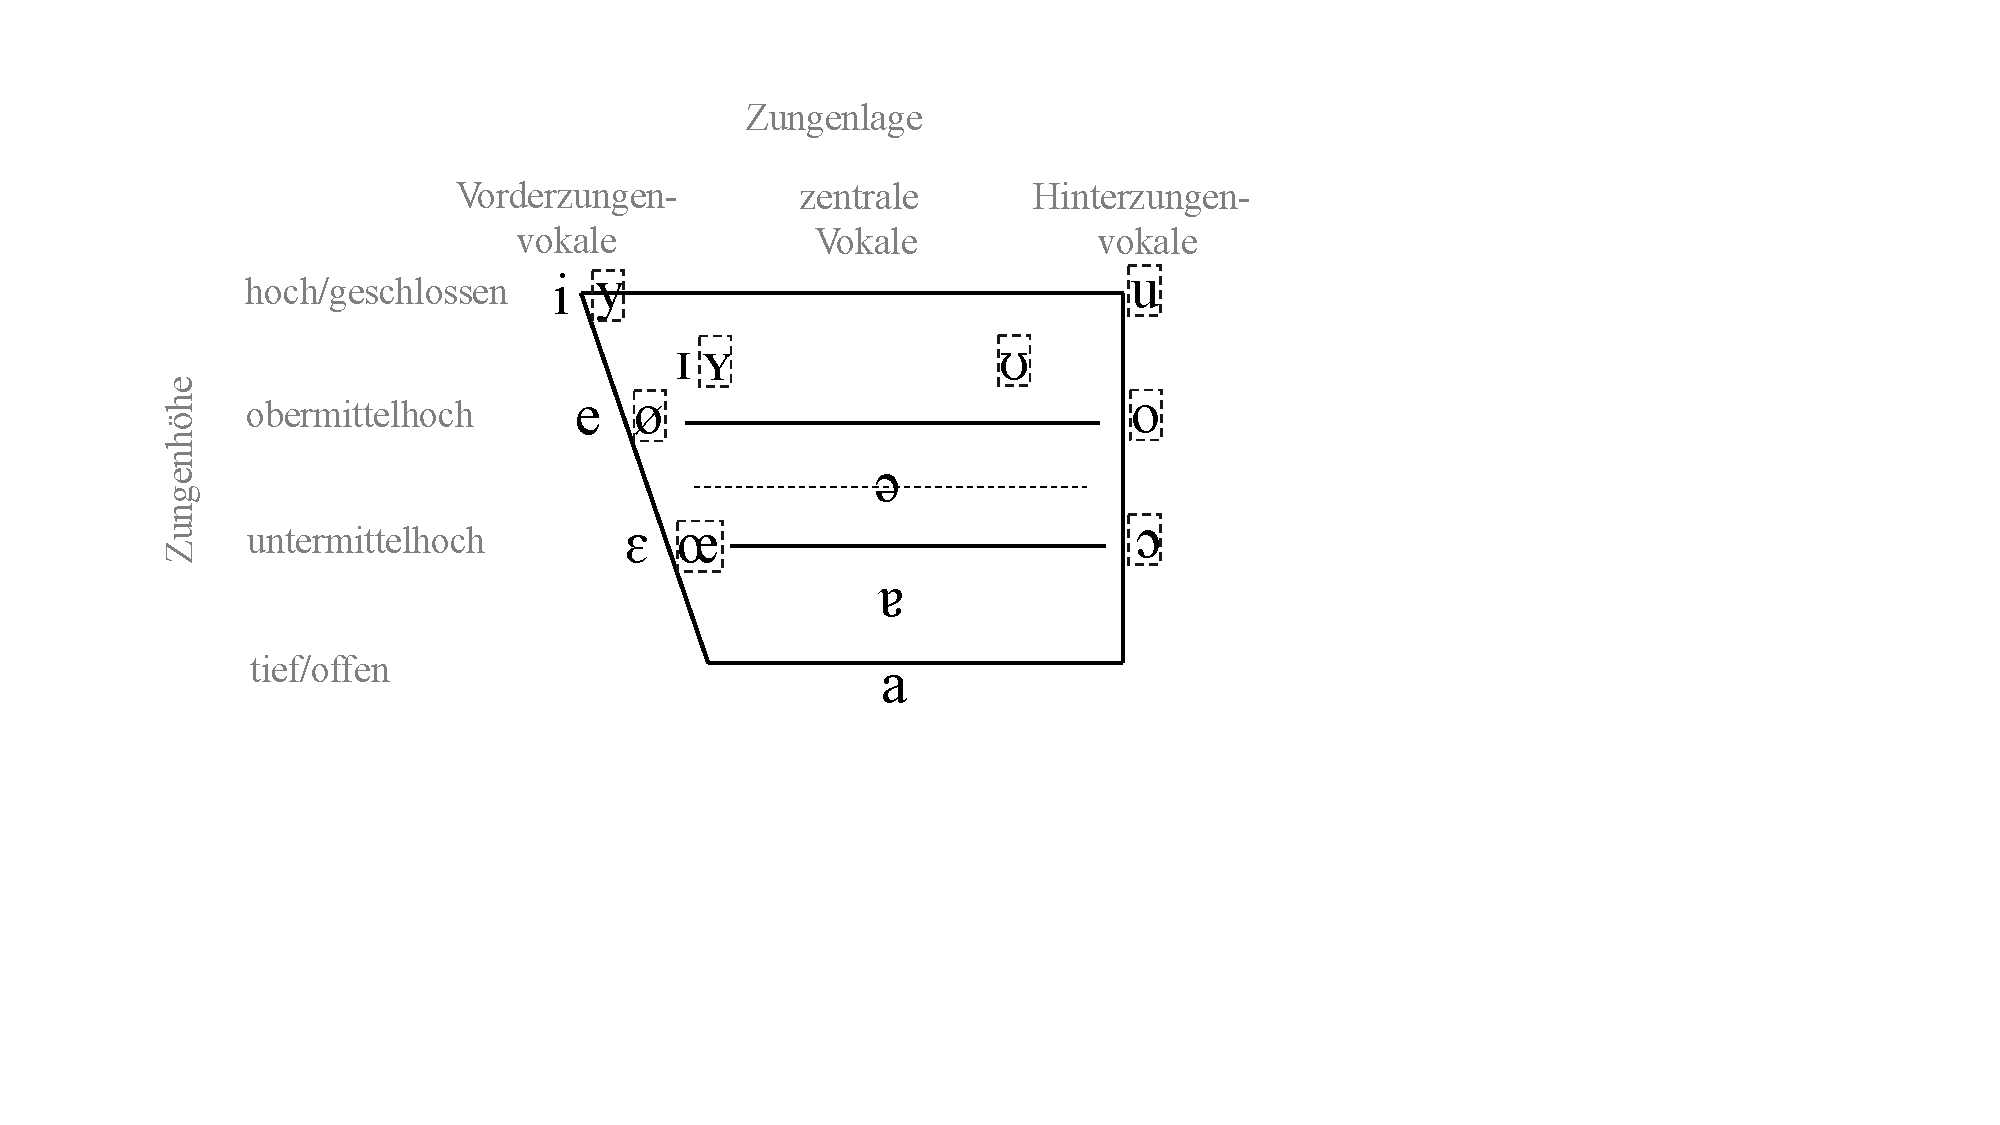
\includegraphics[width=1\textwidth]{figures/Vokalviereck.pdf}
    \caption{Vokalviereck mit den deutschen Vokalen. Gerundete Vokale sind durch ein gestricheltes Kästchen markiert.\label{fig:Vokalviereck}}
\end{figure}

Im Vokalviereck\is{Zungenlage}\is{Vokalviereck}\is{Vorderzungenvokale}\is{Hinterzungenvokal} entspricht die horizontale Dimension der Zungenlage. Ein Laut kann vorn, in der Mitte oder hinten gebildet werden. Die vertikale Dimension entspricht der Zungenhöhe. Ein Laut kann hoch, obermittelhoch, untermittelhoch oder tief sein. Links stehen die Vokale, bei denen die Zunge vorne im palatalen Bereich ist. Diese Vokale werden \textit{Vorderzungenvokale} genannt. Rechts stehen die Vokale, bei denen die Zunge hinten im velaren Bereich ist. Diese Vokale werden \textit{Hinterzungenvokale} genannt. Die Vokale zwischen Vorder- und Hinterzungenvokalen nennt man \textit{zentrale Vokale}.\footnote{Im internationalen phonetischen Alphabet gibt es für die tiefen Vokale das Zeichen \textipa{[a]} für den Vorderzungenvokal und \textipa{[A]} für den Hinterzungenvokal (etwa in Englisch \textit{bath}). Das deutsche \textipa{[a]} in \textit{Bahn} oder \textit{Bann} wird eigentlich zwischen diesen beiden Lauten verortet. Es gibt deshalb phonetisch gesehen keinen guten Grund dafür, das Symbol \textipa{[a]} zu verwenden. Im Gegenteil, phonologisch gesehen, sollte man eher \textipa{[A]} transkribieren, da sich der Laut phonologisch wie ein Hinterzungenvokal verhält. Beispielsweise wird <ch> nach Vorderzungenvokalen \textipa{[\c{c}]} gesprochen, nach \textipa{[a]} aber \textipa{[\textchi ]} \citep[14]{Becker1998}. Dass wir das Symbol \textipa{[a]} verwenden ist also nicht gut begründet, folgt aber den meisten anderen Einführungswerken.}

Um sich die artikulatorischen Unterschiede zu verdeutlichen, kann man versuchen, einen Vorderzungenvokal und einen Hinterzungenvokal ohne Pause nacheinander zu sprechen. Wir wählen den Vorderzungenvokal \textipa{[y]},\footnote{Wir wählen hier \textipa{[y]} statt \textipa{[i]}, weil \textipa{[y]} dieselbe Lippenkonfiguration wie \textipa{[u]} hat und deshalb besser mit \textipa{[u]} verglichen werden kann.} wie im Anlaut von \textit{Übung}, und den Hinterzungenvokal \textipa{[u]}, wie im Anlaut von \textit{Uhu}, und sprechen \textipa{[yyyuuu]}. Dabei kann man beobachten, dass die Zunge am Gaumen von vorn nach hinten gleitet.

Vokale\is{Zungenhöhe}, bei denen die Zunge im Vergleich zu anderen Vokalen relativ hoch liegt, nennt man \textit{hohe Vokale}. In einigen Lehrbüchern findet man auch den Begriff \textit{geschlossene Vokale}. Vokale, bei denen die Zunge sehr weit unten liegt, nennt man \textit{tiefe Vokale} (auch: \textit{offene Vokale}). In der Abbildung sind noch zwei weitere Ebenen eingezeichnet: die \textit{obermittelhohen} und die \textit{untermittelhohen Vokale}. Diese vier Ebenen werden im Folgenden genauer beschrieben.

Wenn man die beiden Vokale \textipa{[i]} und \textipa{[a]} so nacheinander spricht, dass sie ineinander übergehen, kann man feststellen, dass die Zunge -- meist zusammen mit dem Kiefer -- nach unten wandert. Man kan die Vokale \textipa{[i]} wie in \textit{D\underline{ie}b} \textipa{[di:p]}, \textipa{[e]} wie in \textit{\underline{e}ben} \textipa{[\textprimstress Pe:.b@n]}, \textipa{[E]} wie in \textit{B\underline{e}tt} \textipa{[bEt]} und \textipa{[a]} wie in \textit{h\underline{a}ben} \textipa{[\textprimstress ha:.b@n]} oder \textipa{[\textprimstress ha:.b\s{m}]} nacheinander sprechen, sodass ein Vokal in den anderen übergeht: \textipa{[ieEa]}. Dabei bewegt sich die Zunge zusammen mit dem Kiefer nach unten, aber diesmal in vier Schritten. Diese vier Schritte entsprechen den vier Ebenen im Vokalviereck: hoch, obermittelhoch, untermittelhoch, tief.

Dasselbe Experiment kann man für die Hinterzungenvokale machen. Wenn man die Vokale \textipa{[u]} wie in \textit{Hut} \textipa{[hu:t]}, \textipa{[o]} wie in \textit{Mond} \textipa{[mo:nt]}, \textipa{[O]} wie in \textit{oft} \textipa{[POft]} und \textipa{[a]} nacheinander spricht, so dass ein Vokal in den anderen übergeht -- \textipa{[uoOa]} -- wird man feststellen, dass Kiefer und Zunge abgesenkt werden.

Um die anderen Vokale im Vokalviereck beschreiben zu können, braucht man weitere Beschreibungsparameter. 

\subsection{Lippenrundung}
\is{Lippenrundung}
Auffällig ist in Abbildung~\ref{fig:dreiVokale} neben den Unterschieden in der Zungenposition, dass die Lippenkonfiguration zwischen \textipa{[a, i]} und \textipa{[u]} sehr unterschiedlich ist. Bei \textipa{[u]} werden die Lippen nach vorne gestülpt (wie für einen Kuss). Vokale, die mit vorgestülpten Lippen produziert werden, bezeichnet man als \textit{gerundete Vokale}\is{gerundet}. Bei \textipa{[a]} und \textipa{[i]} sind die Lippen nicht gerundet. Solche Vokale bezeichnet man als \textit{ungerundete Vokale}\is{ungerundet}. 

Einige Vokale haben in etwa dieselbe Zungenhöhe und Zungenlage, unterscheiden sich aber in der Lippenrundung. Wenn man den Vokal \textipa{[i]} lange aushält und dann die Lippen rundet, ohne die Zunge zu bewegen, erhält man den Vokal \textipa{[y]} wie in \textit{bügeln} \textipa{[\textprimstress by:.g@ln]}. Wenn man dasselbe mit \textipa{[e]} probiert, erhält man den Vokal \textipa{[\o]}, wie in \textit{Möbel} \textipa{[\textprimstress m\o :.b@l]}. Aus \textipa{[E]}, dem Laut in \textit{Bett}, wird mit Lippenrundung \textipa{[\oe]}, der erste Vokal in \textit{öfter} \textipa{[\textprimstress P\oe f.t5]}.


\subsection{Gespanntheit}
\label{subsection:Gespanntheit}
\is{Gespanntheit}
Der Parameter \textit{Gespanntheit} steht in Relation zur Vokallänge. Die Unterscheidung von \is{Langvokal}\is{Kurzvokal} sogenannten \textit{Lang-} und \textit{Kurzvokalen} spielt im Orthografieerwerb eine wichtige Rolle, denn es gibt spezielle orthografische Markierungen für die beiden Klassen von Lauten. So steht nach einem Kurzvokal häufig (aber längst nicht immer) ein Doppelkonsonant, etwa in \textit{doppelt, Mitte, Rinne}. Ein Langvokal kann durch <ie>, ein stummes h oder einen Doppelvokal gekennzeichnet werden: \textit{schief, Mehl, Saal}. Tabelle~\ref{tab:LangKurzvokale} stellt die beiden Lautklassen gegenüber. \is{Transkription!Längenzeichen}Die Doppelpunkte in den Transkriptionen stehen für die Länge der Langvokale.

\begin{table}
    \centering
        \caption{\label{tab:LangKurzvokale} \gqq{Langvokale} und \gqq{Kurzvokale} im Deutschen mit Beispielwörtern}
    \begin{tabular}{llll}\lsptoprule
         \multicolumn{2}{c}{\gqq{Langvokale}} &\multicolumn{2}{c}{\gqq{Kurzvokale}} \\\midrule
        \textipa{[i:]} & \textit{pieken} \textipa{[\textprimstress pi:.k@n]} & \textipa{[I]}&  \textit{picken} \textipa{[\textprimstress pI\.*{k}@n]}\\
                \textipa{[e:]} & \textit{beten} \textipa{[\textprimstress be:.t@n]} & \textipa{[E]}&  \textit{Betten} \textipa{[\textprimstress bE\.*{t}@n]}\\
                \textipa{[u:]} & \textit{Ruhm} \textipa{[Ku:m]} & \textipa{[U]}&  \textit{Rum} \textipa{[KUm]}\\
                \textipa{[o:]} & \textit{Ofen} \textipa{[\textprimstress Po:.f@n]} & \textipa{[O]}&  \textit{offen} \textipa{[\textprimstress PO\.*{f}@n]}\\
                \textipa{[a:]} & \textit{Bahn} \textipa{[ba:n]} & \textipa{[a]}&  \textit{Bann} \textipa{[ban]}\\
                        \textipa{[y:]} & \textit{Hüte} \textipa{[\textprimstress hy:.t@]} & \textipa{[Y]}&  \textit{Hütte} \textipa{[\textprimstress hY\.*{t}@]}\\
                                \textipa{[\o :]} & \textit{Höhle} \textipa{[\textprimstress h\o :.l@]} & \textipa{[\oe]}&  \textit{Hölle} \textipa{[\textprimstress h\oe \.*{l}@]}\\
        \lspbottomrule
    \end{tabular}
\end{table}



Wenn man die Wörter in Tabelle~\ref{tab:LangKurzvokale} mit gleicher Sprechgeschwindigkeit sprechen und mit einem Mikrophon aufnehmen würde, würde man feststellen, dass die Vokale in den Wörtern in der linken Spalte (die Langvokale), tatsächlich länger sind als die entsprechenden Vokale in den Wörtern in der rechten Spalte (die Kurzvokale). Diese Unterschiede bezeichnet man auch als Unterschiede in der \textit{Vokalquantität}\is{Vokalquantität}.

Die Begriffe Lang- und Kurzvokal sind gut etabliert. \citet{Iivonen1987} und \citet{Spiekermann2002} zeigen, dass der Längenkontrast in Österreich und Süddeutschland auch tatsächlich das hauptsächliche Unterscheidungsmerkmal zwischen den Lautklassen darstellt. In Nord- und Mitteldeutschland beschreibt der Längenunterschied den Kontrast zwischen den beiden Lautklassen aber nur unzureichend. 

Schaut man ins Vokalviereck in Abbildung~\ref{fig:Vokalviereck}, welches sich am norddeutsch geprägten Standard orientiert, stellt man fest, dass die Vokalpaare sich nicht nur durch die Länge, sondern vor allem durch die Zungenposition (Zungenhöhe und Zungenlage) unterscheiden. Diese Unterschiede bezeichnet man auch als Unterschiede in der \textit{Vokalqualität}\is{Vokalqualität}. Der Vokal \textipa{[i]} in \textit{pieken} wird mit höherer Zungenposition und weiter vorne gebildet als der Vokal \textipa{[I]} in \textit{picken}. Der Vokal \textipa{[I]} ist sogar näher am \textipa{[e]} als am \textipa{[i]}. Die Ähnlichkeit zum \textipa{[e]} kann man als Sprecher(in) des norddeutschen Standards auditiv erfahrbar machen, wenn man \textit{picken} langsam vor sich hin spricht, sodass der Vokal gedehnt wird: \mbox{\textit{pi-- --cken}}. Das \textit{pi----} klingt jetzt dem \textit{Pe} in \textit{Pegel} deutlich ähnlicher als dem \textit{pie} in \textit{pieken}. Eigentlich ist das \textipa{[I]} also eher ein gekürztes \textipa{[e]} als ein gekürztes \textipa{[i]}. Deshalb findet man bei Erstklässlern im nordeutschen Raum auch häufig eine Verwechslung von <i> und <e>, etwa <mech> für \textit{mich}.

Das kurze \textipa{[U]} ist artikulatorisch und auditiv näher am langen \textipa{[o:]} als am langen \textipa{[u:]}. Wenn norddeutsche Sprecher \textit{Rum} sehr gedehnt sprechen, hören wir eher \textit{Rom} als \textit{Ruhm}. Dass es Kindern genauso geht, zeigen Schreibungen wie <*mont> für \textit{Mund}, eine Schreibung, die wir schon am Anfang des Kapitels betrachtet haben.

Auch die Schreibung <*höte> für \textit{Hütte} ist in der genannten Varietät darauf zurückzuführen, dass die Lang- und Kurzvokale sich artikulatorisch und akustisch deutlich unterscheiden. Wenn man das \textipa{[Y]} in \textit{Hütte} gedehnt spricht, klingt der Laut eher wie das \textipa{[\o :]} in \textit{Höfe}, aber nicht wie das \textipa{[y:]} in \textit{Hüte}. Das liegt daran, dass die Zunge bei \textipa{[Y]} tiefer als bei \textipa{[y]} liegt.

Die sogenannten Lang- und Kurzvokale unterscheiden sich also in der Länge, aber auch in der Zungenposition, weshalb die Begriffe Lang- und Kurzvokale den Unterschied zumindest für den hier beschriebenen Standard nicht gut erfassen. In der phonetischen Literatur wird der Unterschied deshalb häufig \textit{Gespanntheitsopposition}\is{Gespanntheit} genannt. Die Langvokale werden als \textit{gespannte Vokale} und die Kurzvokale als \textit{ungespannte Vokale} bezeichnet (\zB \cite[39--47]{Becker1998}, \cite[227]{Pompino-Marschall2020}, \cite[26]{FuhrhopPeters2013}, \cite[27]{Hall2000}). Diese Begriffe haben ihren Ursprung in der Annahme, dass für die gespannten Vokale die Zungenmuskeln stärker gespannt sein müssen, weil diese Vokale an extremeren Positionen im Mund gebildet werden (sie stehen weiter außen im Vokalviereck als die ungespannten Partner). Experimentelle Messungen bestätigen das nicht eindeutig, der Begriff Gespanntheit hält sich jedoch \citep[43--44]{Becker1998}. Wir werden die Vokale in der linken Spalte in Tabelle~\ref{tab:LangKurzvokale} deshalb als gespannte Vokale bezeichnen und die in der rechten Spalte als ungespannte Vokale.

Bisher scheint der Unterschied vielleicht vor allem ein terminologischer zu sein: Gespannte Vokale sind nach der bisherigen Diskussion offenbar lange Vokale. Es ist jedoch wichtig, zu verstehen, dass es sich bei vokalischen Kontrasten wie dem zwischen \textit{bieten} und \textit{bitten} zumindest in Nord- und Mitteldeutschland nicht um einen reinen Längenkontrast handelt. Es spricht aber nichts gegen die Verwendung der Termini Lang- und Kurzvokal im Unterricht. \citet[204--207]{Spiekermann2002} zeigt, dass Kinder, die den Kontrast dialektbedingt tatsächlich nur als Längenkontrast produzieren, trotz der Terminologie keinen Vorteil gegenüber Kindern mit eher norddeutscher Aussprache haben.

Anders als die bisherigen Beispiele suggerieren, kann man allerdings von der Gespanntheit eines Vokals nicht sicher auf die Länge des Vokals schließen. Die Vokale, die bisher diskutiert wurden (Tabelle~\ref{tab:LangKurzvokale}), treten alle in betonten Silben auf. Für diese Position kann man tatsächlich sagen, dass die gespannten Vokale lang und die ungespannten kurz sind. In unbetonter Position sind die Verhältnisse anders. Dazu vergleichen wir den ersten Vokal in den Wörtern \textit{leben} und \textit{lebendig}. In beiden Fällen handelt es sich um den gespannten Vokal \textipa{[e]}. Das \textipa{[e]} in \textit{leben} ist aber länger als das \textipa{[e]} in \textit{lebendig}. Das liegt daran, dass \textit{leben} auf der ersten Silbe betont ist, \textit{lebendig} aber auf der zweiten. In betonter Position werden gespannte Vokale also gelängt. Man transkribiert deshalb \textit{leben} \textipa{[\textprimstress le:.b@n]} mit einem Doppelpunkt\is{Transkription!Längenzeichen}, der die Länge signalisiert, und \textit{lebendig} \textipa{[le\textprimstress bEn.dI\c{c}]} oder \textipa{[le\textprimstress bEn.dIk]} ohne Doppelpunkt.

Gespannte Vokale sind also nicht immer lang, sondern sie sind nur in betonter Position lang. Deshalb ist der Terminus Langvokal für diese Vokale nicht immer zutreffend.

Bei den ungespannten Vokalen gibt es keinen deutlichen Längenunterschied zwischen betonten und unbetonten Vokalen. Dazu vergleichen wir das \textipa{[E]} in \textit{Bäcker} und \textit{Bäckerei}. \textit{Bäcker} ist auf der ersten Silbe betont, aber das \textipa{[E]} ist kurz. \textit{Bäckerei} ist auf der letzten Silbe betont, und das \textipa{[E]} ist kurz. Man transkribiert deshalb: \textipa{[\textprimstress bE\.*k5]} und \textipa{[bE\.*k@\textprimstress K\t*{aI}]}.

Man kann also drei Gruppen von Vokalen unterscheiden \citep[120--121]{Jessen2010}: 
\begin{itemize}
    \item die gespannten langen Vokale
    \item die gespannten kurzen Vokale
    \item die ungespannten Vokale
\end{itemize}

Tabelle~\ref{tab:GespanntUngespannt} besteht deshalb im Gegensatz zu Tabelle~\ref{tab:LangKurzvokale} aus drei Spalten, nämlich den beiden äußeren, die wir aus Tabelle~\ref{tab:LangKurzvokale} kennen, und einer neuen mittleren Spalte für die gespannten Vokale in unbetonten Silben.

\begin{table}
    \centering
%\resizebox{\textwidth}{!}{
\oneline{
    \begin{tabular}{llllll}\lsptoprule
         \multicolumn{2}{c}{gespannte lange Vokale} & \multicolumn{2}{c}{gespannte kurze Vokale} &\multicolumn{2}{c}{ungespannte Vokale} \\\midrule
        \textipa{[i:]} & \textit{pieken} \textipa{[\textprimstress pi:.k@n]} &\textipa{[i]} & \textit{Zitrone} \textipa{[\t{ts}i\textprimstress tKo:.n@]}  & \textipa{[I]}&  \textit{picken} \textipa{[\textprimstress pI\.*k@n]}\\
                \textipa{[e:]} & \textit{beten} \textipa{[\textprimstress be:.t@n]} &\textipa{[e]} & \textit{lebendig} \textipa{[le\textprimstress bEn.dI\c{c}]} & \textipa{[E]}&  \textit{Betten} \textipa{[\textprimstress bE\.*t@n]}\\
                \textipa{[u:]} & \textit{Ruhm} \textipa{[Ku:m]} & \textipa{[u]}& \textit{Museum} \textipa{[mu\textprimstress ze:.Um]} &\textipa{[U]} &  \textit{Rum} \textipa{[KUm]}\\
                \textipa{[o:]} & \textit{Ofen} \textipa{[\textprimstress Po:.f@n]} &\textipa{[o]} & \textit{Modell} \textipa{[mo\textprimstress dEl]} & \textipa{[O]}&  \textit{offen} \textipa{[\textprimstress PO\.*f@n]}\\
                        \textipa{[y:]} & \textit{Hüte} \textipa{[\textprimstress hy:.t@]} &\textipa{[y]} & \textit{Myom} \textipa{[my\textprimstress o:m]} & \textipa{[Y]}&  \textit{Hütte} \textipa{[\textprimstress hY\.*t@]}\\
                                \textipa{[\o :]} & \textit{Höhle} \textipa{[\textprimstress h\o :.l@]} &\textipa{[\o ]} & \textit{Ödem} \textipa{[P\o \textprimstress de:m]} & \textipa{[\oe]}&  \textit{Hölle} \textipa{[\textprimstress h\oe \.*l@]}\\
                                \cmidrule(r){1-4}\cmidrule(l){5-6}
          \multicolumn{4}{c}{peripher} &  \multicolumn{2}{c}{zentral}\\
        \cmidrule(r){1-2}\cmidrule(l){3-6}
            \multicolumn{2}{c}{lang} &  \multicolumn{4}{c}{kurz}\\\lspbottomrule
    \end{tabular}
    }
 \caption{Einteilung der deutschen Vokale in gespannt/ungespannt und lang/kurz}
        \label{tab:GespanntUngespannt}
\end{table}

Die Vokale in der linken und mittleren Spalte sind gespannt und haben also eine \textit{periphere} (extremere) Zungenposition. Sie werden mit demselben Symbol transkribiert, da die Zungenposition vergleichbar ist. Die Vokale in der rechten Spalte haben eine \textit{zentralere} Zungenposition (eher mittig). Sie werden deshalb mit einem anderen Symbol transkribiert. Die Vokale in der linken Spalte sind lang und werden deshalb \is{Transkription!Längenzeichen}mit Doppelpunkt transkribiert. Die Vokale in den beiden anderen Spalten sind kurz und werden deshalb ohne Doppelpunkt transkribiert.

Es ist auffällig, dass native Wörter vor allem in der linken und rechten Spalte zu finden sind. Typischerweise kommen gespannte Vokale vor allem in betonten Silben vor. In die mittlere Kategorie fallen vor allem Fremdwörter. Es ist wichtig, diese Kategorie identifizieren zu können, da bei diesen Wörtern die deutschen Orthografieregeln für die gespannten Vokale nicht angewandt werden können. Beispielsweise gibt es bei diesen Wörtern kein <ie> und auch kein Dehnungs-\textit{h}. Kindliche Schreibungen wie <*Zietrone> oder <*Tehater>, bei denen die Regeln für die gespannten Langvokale angewandt werden, sind darauf zurückzuführen, dass die Kinder die Vokale als gespannt wahrnehmen.

Zwischen den Vokalen \textipa{[a]} in \textit{Bann} und \textipa{[a:]} in \textit{Bahn} gibt es laut \citet[14--15]{Becker1998} einen messbaren, aber keinen hörbaren Unterschied in der Vokalqualität. Sie unterscheiden sich also nur in der Vokalquantität und sind deshalb in Tabelle~\ref{tab:GespanntUngespannt} nicht enthalten.


Vor allem in der Bildungssprache\footnote{Unter Bildungssprache verstehen wir hier \citet[]{Habermas1977} folgend ein sprachliches Register, welches in Bildungsinstitutionen verwendet wird und welches allgemein zur Bildungsaneignung verwendet wird.} wird \citet[15--16]{Becker1998} zufolge häufig ein Unterschied zwischen \textipa{[E:]}, wie in \textit{Dänen}, und \textipa{[e:]}, wie in \textit{dehnen}, gemacht. Außerhalb von Bildungskontexten ist diese Unterscheidung in Nord- und Ostdeutschland und in Ostösterreich laut \citet[67]{DudenAussprache2023} jedoch kaum zu hören, beide Wörter werden \textipa{[\textprimstress de:n@n]} oder \textipa{[\textprimstress de:n\s{n}]} gesprochen. Auch in anderen deutschsprachigen Gebieten fallen die beiden Laute bei vielen Sprechern zusammen. Lediglich in der Schweiz wird konsequent zwischen \textipa{[E:]} und \textipa{[e:]} unterschieden \citep[67]{DudenAussprache2023}. Laut Ausspracheduden sind beide Varianten standardgemäß, das \citet[138]{DudenZweifelsfaelle2021} empfiehlt die Aussprache \textipa{[E:]}, \zB in \textit{Träne} \textipa{[\textprimstress tKE:.n@]} statt \textipa{[\textprimstress tKe:.n@]}.

\largerpage
  In (\ref{väter}) bis (\ref{gewähren}) sind weitere Beispiele gegeben, bei denen es eine Diskrepanz zwischen dem gibt, was laut \citet{DudenZweifelsfaelle2021} empfohlen wird (erste Transkription bei jedem Beispiel) und der Lautung, die in weiten Teilen Deutschlands und Österreichs produziert wird (zweite Transkription). 
\ea
\ea \label{väter}Väter: \textipa{[\textprimstress fE:.t5]} vs. \textipa{[\textprimstress fe:.t5]}
\ex \label{mädchen}Mädchen: \textipa{[\textprimstress mE:t.\c{c}@n]} vs. \textipa{[\textprimstress me:t.\c{c}@n]}
\ex \label{ähnlich}ähnlich: \textipa{[\textprimstress PE:n.lI\c{c}]} vs. \textipa{[\textprimstress Pe:n.lI\c{c}]}
\ex \label{käse}Käse: \textipa{[\textprimstress kE:.z@]} vs. \textipa{[\textprimstress ke:.z@]}
\ex \label{gewähren}gewähren: \textipa{[g@\textprimstress vE:.K@n]} vs. \textipa{[g@\textprimstress ve:.K@n]}
\z
\z

\citet[14--15 und Quellen darin]{Becker1998} zufolge hat die \textipa{[E:]}-Aussprache ihren Ursprung in der Schriftsprache, wo zwischen <e> und <ä> unterschieden wird. Die einzigen Fälle, in denen viele Sprecherinnen und Sprecher tatsächlich häufig \textipa{[E:]} sprechen, sind Wörter, deren Aussprache sonst mit der anderer Wörter zusammenfallen würde, etwa \textit{sehen--sähen, geben--gäben} und das zuvor erwähnte \textit{dehnen--Dänen}.


\subsection{Reduktionsvokale}\label{subsection:Reduktionsvokale}

Alle Vokale, die bisher diskutiert wurden, können den Nukleus einer betonten Silbe bilden. Es gibt jedoch auch Vokale, die das nicht können. Diese Vokale nennt man \textit{Reduktionsvokale}. Im Deutschen gibt es zwei Reduktionsvokale, den \textit{Schwa-Laut} \textipa{[@]} und das \textit{tiefe Schwa} \textipa{[5]}, auch \textit{a-Schwa} oder \textit{Lehrer-Schwa} genannt. 

Das Schwa \is{Laute!Schwa} \textipa{[@]} wird orthografisch <e> geschrieben und kommt im Standarddeutschen nur in unbetonten Silben vor, wie in den Beispielen (\ref{ex:Lage}) und (\ref{ex:geteilt}). Im Vokalviereck steht der Schwa-Laut direkt im Zentrum (vgl. Abbildung \ref{fig:Vokalviereck}). Er wird gebildet, indem die Zunge entspannt im Mund liegt.

\ea
\ea \label{ex:Lage} Lage \textipa{[\textprimstress la:.g@]}
\ex \label{ex:geteilt} geteilt \textipa{[g@\textprimstress t\t*{aI}lt]}
\z 
\z

Im Standarddeutschen kommt er außerdem in förmlicher Rede in der Infinitivendung der Verben vor, wie in Beispiel (\ref{ex:lesen}), aber auch in vielen anderen Endsilben, wie in Beispiel (\ref{ex:Mantel}). An diesen Stellen wird er in fließender Rede jedoch oft getilgt (sogenannte Schwa-Tilgung, vgl. Abschnitt~\ref{sec:Schwatilgung}).

\ea
\ea \label{ex:lesen} \textit{lesen}, explizit: \textipa{[\textprimstress le:.z@n]}, in fließender Rede: \textipa{[\textprimstress le:.z\s{n}]}
\ex \label{ex:Mantel} \textit{Mantel}, explizit: \textipa{[\textprimstress man.t@l]}, in fließender Rede: \textipa{[\textprimstress man.t\s{l}]}\footnote{Ein Strichlein unter einem Konsonanten bedeutet, dass der Konsonant silbisch ist. Er übernimmt also die Nukleus-Funktion, die sonst von einem Vokal wahrgenommen wird.}
\z 
\z


Das \is{Laute!tiefes Schwa} tiefe Schwa \textipa{[5]} wird <r> oder <er> geschrieben. Wenn es zusammen mit einem anderen Vokal den Nukleus bildet, wie in Bespiel (\ref{ex:für}), wird es <r> geschrieben. Wenn es alleine den Nukleus bildet, wie in den Beispielen (\ref{ex:Drucker}) und (\ref{ex:verbinden}) wird es <er> geschrieben. 

\ea
\ea \label{ex:für} für \textipa{[fy5]} 
\ex \label{ex:Drucker} Drucker \textipa{[\textprimstress drU\.*k5]}
\ex \label{ex:verbinden} verbinden \textipa{[f5\textprimstress bIn.d@n]}
\z 
\z

Das tiefe Schwa \textipa{[5]} und das Schwa \textipa{[@]} sind bedeutungsunterscheidend, wie die Beispiele (\ref{ex:Lehre-Lehrer}) und (\ref{ex:meiste-Meister}) zeigen.\footnote{Solche Beispiele, die sich nur durch einen einzigen Laut unterscheiden, nennt man Minimalpaare (vgl. Abschnitt~\ref{sec:Allophone}.)}

\ea
\ea \label{ex:Lehre-Lehrer} Lehre -- Lehrer \textipa{[\textprimstress le:.K@} -- \textipa{\textprimstress le:.K5]}
\ex \label{ex:meiste-Meister} meiste -- Meister \textipa{[\textprimstress m\t*{aI}s.t@} -- \textipa{\textprimstress m\t*{aI}s.t5]}
\z 
\z


Im Vokalviereck steht das tiefe Schwa zwischen Schwa und \textipa{[a]} (vgl. Abbildung \ref{fig:Vokalviereck} auf Seite \pageref{fig:Vokalviereck}). Akustisch ist es dem \textipa{[a]} sehr ähnlich, weshalb man bei Schreibanfängern häufig a-Schreibungen findet: <*füa> (\textit{für}), <*Kinda> (\textit{Kinder}). \citet[42]{RathckeMooshammer2020} zeigen, dass Minimalpaare wie in den Beispielen (\ref{ex:Cola}), (\ref{ex:Feta}) und (\ref{ex:Opa}) in den nördlichen Regionen Deutschlands nicht unterscheidbar produziert werden. 

\ea
\ea \label{ex:Cola} Cola \textipa{[\textprimstress ko:.la]} vs. Kohler \textipa{[\textprimstress ko:.l5]}
\ex \label{ex:Feta} Feta \textipa{[\textprimstress fe:.ta]} vs. Väter \textipa{[\textprimstress fe:.t5]}
\ex \label{ex:Opa} Opa \textipa{[\textprimstress Po:.pa]} vs. Oper \textipa{[\textprimstress Po:.p5]} 
\z 
\z


Wenn, wie in Beispiel (\ref{ex:für}), das tiefe Schwa zusammen mit einem anderen Vokal in einer Silbe steht, bildet es mit diesem Vokal zusammen einen \is{Diphthong}Diphthong (vgl. Abschnitt~\ref{subsec:Diphthonge}). 

Vor allem nach ungespannten Vokalen kann statt des tiefen Schwas ein r-Laut gesprochen werden. Das kann man etwa bei der Aussprache von \textit{Erde} beobachten \citep[308]{DudenAussprache2023}. In Dialektregionen, wo der Vokal gespannt gesprochen wird, wird das tiefe Schwa bevorzugt: \textipa{[\textprimstress Pe:5.d@]}, wenn der Vokal  ungespannt gesprochen wird, folgt ihm eher ein r-Laut: \textipa{[\textprimstress PEr.d@]}.

\subsection{Diphthonge}
\label{subsec:Diphthonge}
\largerpage
Vokale können in \textit{Monophthonge}\is{Monophthong} und \textit{Diphthonge}\is{Diphthong} eingeteilt werden. Alle Vokale, die bisher besprochen wurden, \zB \textipa{[i, a, u]}, sind Monophthonge. Bei Monophthongen bewegt sich die Zunge in eine bestimmte vokalische Position und dann bewegt sie sich zum Koda-Konsonanten oder einem Laut in der nächsten Silbe.

Diphthonge (auch \textit{Zwielaute}\is{Diphthong!Zwielaut} genannt) sind einsilbige Verbindungen aus zwei vokalischen Segmenten, also zwei Segmenten, die zusammen einen Nukleus bilden, \zB \textipa{[\t*{aU}]}. In Tabelle~\ref{tab:EinsilbigZweisilbig} sind zweisilbige und einsilbige Vokalkombinationen gegenübergestellt. \textit{Lea} ist ein zweisilbiges Wort, \textipa{[e]} und \textipa{[a]} gehören zu zwei unterschiedlichen Silben und sind daher Monophthonge. \textit{leer} ist akustisch sehr ähnlich, aber einsilbig, da das Wort den Diphthong \textipa{[\t*{e5}]} enthält. \textipa{[e]} und \textipa{[5]} gehören zur selben Silbe. 

\begin{table}
    \centering
        \caption{\label{tab:EinsilbigZweisilbig} Zweisilbige (erste Spalte) und einsilbige (zweite Spalte) Vokalverbindungen.}
    \begin{tabular}{ll}\lsptoprule
        zweisilbig & einsilbig \\\midrule
        \textit{Lea} \textipa{[\textprimstress le:.a]}& \textit{leer} \textipa{[l\t*{e5}]}\\
        \textit{Pia} \textipa{[\textprimstress pi:.a]}& \textit{ihr} \textipa{[P\t*{i5}]}\\
        \textit{Laos} \textipa{[\textprimstress la:.Os]}& \textit{Laus} \textipa{[l\t*{aU}s]}\\
        \textit{stoisch} \textipa{[\textprimstress Sto:.IS]}& \textit{Streu} \textipa{[StK\t*{OI}]}
    \\\lspbottomrule
    \end{tabular}
\end{table}

Diphthonge werden gebildet, indem die Zunge aus der Position eines Vokals in die Position eines anderen Lautes übergeht, beim \textipa{[\t*{aU}]} etwa vom \textipa{[a]} zum \textipa{[U]}. Diphthonge werden meist mit einem Bogen unter den beiden Segmenten trans\-kribiert.

Die Diphthonge können eingeteilt werden in \textit{schließende} (auch \textit{steigende})\is{Diphthong!schließend} und \textit{zentralisierende} Diphthonge. Bei schließenden Diphthongen bewegt sich die Zunge von einer offeneren in eine geschlossenere Position, was auf den Grad der Öffnung bzw. Schließung des Mundes abzielt. Im Deutschen gibt es die drei schließende Diphthonge, \textipa{[\t*{aI}]} wie in \textit{Eis}, \textipa{[\t*{aU}]} wie in \textit{aus} und \textipa{[\t*{OI}]}) wie in \textit{euch}.\footnote{Anmerkung zur Transkription: Bei den schließenden Diphthongen erreicht die Zunge im Deutschen nie den gespannten Vokal. Deshalb tranksribieren die meisten Autor(innen) nicht mit gespannten Vokalen als zweitem Element: \textipa{[\t*{ai}, \t*{au}, \t*{Oi}]}, cf. aber \citet[117--118]{Becker1998}. Die Position, die die Zunge beim zweiten Segment erreicht, ist relativ variabel, weshalb einige Autorinnen und Autoren statt \textipa{[\t*{aI}]} \textipa{[\t*{ae}]} oder \textipa{[\t*{aE}]} transkribieren und statt \textipa{[\t*{aU}]} \textipa{[\t*{ao}]} oder \textipa{[\t*{aO}]}, cf. \citet[27]{FuhrhopPeters2013}, \citet[101]{Schaefer2018_3Aufl}. Bei \textipa{[\t*{OI}]} wird die Lippenrundung auf das zweite Segment übertragen, sodass man auch die Transkriptionen \textipa{[\t*{OY}, \t*{O\o}]} oder (seltener) sogar \textipa{[\t*{O\oe}]} findet. \citet{PaetzoldSimpson1997} zeigen mittels akustischer Messungen, dass Frauen die Diphthonge anders produzieren als Männer. Frauen produzieren das zweite Segment in der Regel geschlossener als Männer. \citet{WeirichSimpson2018} bestätigen das für \textipa{[\t*{aI}]} mit artikulatorischen Daten. Für Frauen wären diesen Studien zufolge wohl die Transkriptionen \textipa{[\t*{aI}, \t*{aU}]} und \textipa{[\t*{OI}]} am zutreffendsten, für Männer hingegeben \textipa{[\t*{aE}, \t*{ao}, \t*{OY}]}.}

Bei zentralisierenden Diphthongen\is{Diphthong!zentralisierend} bewegt sich die Zunge auf einen zentralen Vokal hin. Alle zentralisierenden Diphthonge im Deutschen sind Kombinationen aus einem Vokal und dem tiefen Schwa, \zB \textipa{[\t*{e5}, \t*{o5}, \t*{u5}]} in \textit{er, Ohr, Uhr}. Deshalb werden sie auch \textit{r-Diphthonge} genannt. \is{Diphthong!zentralisierend!r-Diphthonge}

Einige Autorinnen und Autoren\is{Transkription!Längenzeichen} transkribieren die r-Diphthonge (also die zentralisierenden Diphthonge), bei denen der erste Bestandteil ein gespannter Vokal ist, mit Längenmarkierung: \textipa{[e:5, o:5, u:5]} \citep[28]{FuhrhopPeters2013}. Die Längenmarkierung kann man phonetisch nicht begründen; die r-Diphthonge sind nicht länger als die schließenden Diphthonge. Man kann jedoch argumentieren, dass das tiefe Schwa phonologisch ein zugrundeliegender Konsonant ist. Wenn man außerdem der Regel folgt, dass gespannte Vokale in betonter Position lang sind, ist der Doppelpunkt berechtigt (vgl. Abschnitt~\ref{subsection:Gespanntheit}). 

Unterschiedliche Transkriptionen findet man auch bei r-Diphthongen mit ungespanntem ersten Segment. Während \citet[28]{FuhrhopPeters2013} die Diphthonge in \textit{Herr, dürr} und \textit{dörr} \textipa{[E5, Y5, \oe 5]} transkribieren,  gibt das \citet{DudenAussprache2023} die Transkriptionen \textipa{[hEr, dYr, d\oe r]} an. Auch \citet[33--34]{Ruesetal2014} sehen das tiefe Schwa nur nach gespannten Vokalen vor. Kindliche Schreibungen wie <leant> für \textit{lernt} und <wode> für \textit{wurde}\footnote{Karlsruhe Children's Text Corpus \citep{Lavalleyetal2015}.} suggerieren jedoch, dass auch nach ungespannten Vokalen \textipa{[5]} möglich ist.

Für den Orthografieerwerb relevant sind die Diphthonge aus mehreren Gründen. Nur einer der steigenden Diphthonge ist unproblematisch, nämlich der Diph\-thong \textipa{[\t*{aU}]}. Für den Diphthong \textipa{[\t*{aI}]} gibt es zwei Schreibungen, <ei> und <ai>, von denen das seltenere <ai> phonetisch schlüssig ist, sodass Lernende es zu Beginn des Schriftspracherwerbs vorziehen. Für \textipa{[\t*{OI}]} gibt es ebenfalls zwei Schreibungen, <eu> und <äu>. Die zweite Schreibung lässt sich nur morphologisch erklären. Morphologisch bedeutet hier, dass die Schreibung auf die Verwandtschaft mit Wörtern mit <au> zurückzuführen ist, etwa \textit{Häuser} auf \textit{Haus} (vgl. Abschnitt~\ref{subsec:ääuSchreibungen}). Der Diphthong \textipa{[\t*{OI}]} wird zu Beginn des Schriftspracherwerbs oft <oi> geschrieben, weil diese Schreibung phonetisch schlüssig ist.\footnote{Die Schreibung <eu> für \textipa{[OI]}, die wir heute verwenden, geht auf den mittelhochdeutschen Diphthong \textipa{[iu]} zurück, für den die Schreibung <eu> existierte, um ihn von der umgelauteten Variante von \textipa{[iu]}, nämlich \textipa{[y:]}, zu unterscheiden. \textipa{[iu]} wurde im Zuge der neuhochdeutschen Diphthongierung zu \textipa{[OI]}, cf. \citet[74, 100]{Paul2007}.}

%\addsec{Exkurs: Wahrnehmung der Silbenanzahl}
\begin{Exkurs}{Wahrnehmung der Silbenanzahl}\label{ex:Silbenanzahl}

\largerpage
Woher weiß man, dass \textit{Lea} zweisilbig ist und \textit{leer} einsilbig? Silben sind psycholinguistische Einheiten. Das äußert sich zum Beispiel darin, dass die Wahrnehmung der Anzahl von Silben kategorial ist, selbst wenn der Input ein Kontinuum ist. \citet{Jannedy1994} hat Versuchspersonen ein Kontinuum von \textit{braten} zu \textit{beraten} präsentiert. Die Versuchspersonen hörten also \textit{braten} ohne Schwa zwischen \textipa{[b]} und \textipa{[K]}, und außerdem noch Produktionen mit unterschiedlich langem Schwa. Abhängig von der Versuchsperson und der Sprechgeschwindigkeit hörten die Versuchspersonen immer entweder \textit{braten}, den Zweisilber, oder \textit{beraten}, den Dreisilber.

Denselben Effekt kann man auch für Diphthonge versus Hiatus (Abfolge von zwei Vokalen) zeigen. Ein Hiatus (in unserem Beispiel \textit{Lea)} unterscheidet sich von einem Diphthong (in unserem Beispiel \textit{leer}) vor allem dadurch, dass er länger dauert und extremere artikulatorische Positionen verwendet werden \citep{Aguilar1999}. Wenn man mit diesen Ankerpunkten ein Kontinuum erstellt, hören die Versuchspersonen wieder kategorial, also entweder den Diphthong oder den Hiatus, obwohl der Input nicht kategorial ist. 
\end{Exkurs}

\section{Zusammenfassung Phonetik}\label{sec:ZusfassKons}
\largerpage
\begin{table}[b]
    \centering
        \caption{\label{tab:IPA_Kons} Standarddeutsches Konsonanteninventar (inklusive Allophonen). Spalten: Artikulationsorte. Zeilen: Artikulationsarten: Stimmlose Konsonanten stehen links in einer Zelle, stimmhafte stehen rechts.}
        \oneline{
    \begin{tabular}{llllllllllllllllllllllll}\lsptoprule
         &\multicolumn{2}{c}{\rotatebox{90}{bilabial}} &&\multicolumn{2}{c}{\rotatebox{90}{labiodental}} && \multicolumn{2}{c}{\rotatebox{90}{alveolar}} && \multicolumn{2}{c}{\rotatebox{90}{postalveolar}} && \multicolumn{2}{c}{\rotatebox{90}{palatal}} && \multicolumn{2}{c}{\rotatebox{90}{velar}} && \multicolumn{2}{c}{\rotatebox{90}{uvular}} && \multicolumn{2}{c}{\rotatebox{90}{glottal}}\\\midrule

        Plosive& \textipa{p}& \textipa{b} &\textipa{ }&&&\textipa{ } & \textipa{t} &\textipa{d}&\textipa{ } &&&\textipa{ }& & &\textipa{ }& \textipa{k} &\textipa{g} &\textipa{ }&&&\textipa{ }& \textipa{P}&\\

        Frikative &&&& \textipa{f} & \textipa{v} && \textipa{s} & \textipa{z} & &\textipa{S} &  \textipa{Z} && \textipa{\c{c}} &&& x&&& \textipa{\textchi}& {\raggedright \textipa{\textinvscr}}& &\textipa{h}&\\

       Nasale && \textipa{m} && &&&& \textipa{n} &&&& & && &&\textipa{N} &&& & &\\

        Vibranten &&&&&&&& \arraybackslash \textipa{r}& &&&&&&&&&&& \textscr &&\\

        Approximanten && & & & &&&&&&&&& \textipa{j}& & &&&& \\

        Laterale && && &&&& \textipa{l} & & & &&&&&&&        \\\lspbottomrule
    \end{tabular}
    }
\end{table}
Bevor wir uns im nächsten Kapitel mit der Phonologie des Deutschen beschäftigen, fassen wir die wesentlichen Punkte zum Thema Phonetik in Stichpunkten zusammen. Außerdem finden Sie hier die für die Betrachtung des Deutschen wichtigen IPA-Zeichen in Tabellen zusammengefasst.
\begin{itemize}

\item Laute können in Konsonanten und Vokale eingeteilt werden. Konsonanten können nach Stimmhaftigkeit, Artikulationsort und Artikulationsart klassifiziert werden. In der Konsonantenübersicht des internationalen phonetischen Alphabets sind in den Spalten die unterschiedlichen Artikulationsorte angegeben und in den Zeilen die Artikulationsarten. Stimmlose Laute stehen links, stimmhafte stehen rechts in den jeweiligen Feldern. Tabelle~\ref{tab:IPA_Kons} listet die für das Deutsche relevanten Symbole auf. Tabelle~\ref{tab:Kons_Beispielwörter} gibt Beispielwörter für die einzelnen Laute an.

\begin{table}[t]
    \small
        \caption{\label{tab:Kons_Beispielwörter} Beispielwörter für die einzelnen Konsonanten. Die Beispiele demonstrieren die häufigsten orthografischen Verschriftungen.}
    \begin{tabularx}{\textwidth}{Xlll}\lsptoprule
    \multicolumn{2}{c}{Obstruenten} & \multicolumn{2}{c}{Sonoranten}\\\midrule
     \textipa{[p]} & \textit{P}anne \textipa{[\textprimstress pa\.*{n}@]}&   \textipa{[m]} & \textit{M}ensch \textipa{[mEnS]}  \\
     \textipa{[b]} & \textit{B}ein \textipa{[b\t*{aI}n]} &  \textipa{[n]} & \textit{N}ase \textipa{[\textprimstress na:.z@]}\\
     \textipa{[t]} & \textit{T}eich  \textipa{[t\t*{aI}\c{c}]}  &  \textipa{[N]} & e\textit{ng} \textipa{[PEN]} \\
     \textipa{[d]} & \textit{D}eich  \textipa{[d\t*{aI}\c{c}]}&  \textipa{[r]} & \textit{r}eich \textipa{[r\t*{aI}\c{c}]} \\
     \textipa{[k]} & \textit{K}ohl \textipa{[ko:l]} &   \textipa{[\textscr]} & \textit{r}eich \textipa{[\textscr \t*{aI}\c{c}]} \\
     \textipa{[g]} & \textit{G}ans \textipa{[gans]}  & \textipa{[j]} & \textit{j}eder \textipa{[\textprimstress je:.d5]}\\
     \textipa{[P]} & Be\textit{\_}amter \textipa{[b@\textprimstress Pam.t5]}   & \textipa{[l]} & \textit{l}eise \textipa{[\textprimstress l\t*{aI}.z@]}\\
    \textipa{[f]}& \textit{F}aden \textipa{[\textprimstress fa:.d@n]},\textit{V}ater \textipa{[\textprimstress fa:.t5]}&&\\
    \textipa{[v]} &\textit{W}ein  \textipa{[v\t*{aI}n]}, \textit{V}ase \textipa{[\textprimstress va:.z@]}&&\\
     \textipa{[s]}& Me\textit{ss}e  \textipa{[\textprimstress mE\.*s@]}, Bu\textit{s} \textipa{[bUs]}, Stra\textit{ß}e \textipa{[\textprimstress StKa:.s@]}&&\\
  \textipa{[z]} & \textit{S}onne \textipa{[\textprimstress zO\.*n@]}&&\\
     \textipa{[S]}& \textit{Sch}ule \textipa{[\textprimstress Su:.l@]}&&\\
 \textipa{[Z]} & \textit{G}enie \textipa{[Ze\textprimstress ni:]}&&\\
   \textipa{[\c{c}]}& E\textit{ch}o \textipa{[\textprimstress PE\.*{\c{c}}o]}&&\\
    \textipa{[x]} & Bu\textit{ch} \textipa{[bu:x]}&&\\
   \textipa{[X]} & Ba\textit{ch} \textipa{[baX]}&&\\
   \textipa{[K]} & \textit{r}eich \textipa{[K\t*{aI}\c{c}]}&&\\
\textipa{[h]} & \textit{h}eiß \textipa{[h\t*{aI}s]}&&\\
 \textipa{[\t{pf}]} & hü\textit{pf}en \textipa{[\textprimstress hY\.*{\t{pf}}@n]}&&\\
  \textipa{[\t{tS}]} & kla\textit{tsch}en \textipa{[\textprimstress kla\.*{\t{tS}}@n]}&&\\
\textipa{[\t{ts}]} & Hi\textit{tz}e \textipa{[\textprimstress hI\.*{\t{ts}}@]}, Hol\textit{z} \textipa{[\textprimstress hOl\t{ts}]}&&\\
   \lspbottomrule
    \end{tabularx}
\end{table}

\item Vokale sind stimmhaft. Sie können nach Zungenhöhe, Zungenlage, Lippenrundung und Gespanntheit eingeteilt werden. Zungenhöhe und Zungenlage sind im Vokalviereck dargestellt (vgl. Abbildung~\ref{fig:Vokalviereck}). Alle Hinterzungenvokale sind gerundet. Im Deutschen gibt es vier gerundeten Vorderzungenvokale: \textipa{[y, Y, \o , \oe ]}. Die meisten Vokale kommen in Paaren (gespannt vs. ungespannt) vor. Gespannte Vokale in betonter Position sind lang. Diese Vokale werden mit einem Längenzeichen transkribiert. Alle anderen Vokale sind kurz. 

\item Im Deutschen gibt es zwei Reduktionsvokale, das Schwa \textipa{[@]} und das tiefe Schwa \textipa{[5]}. Der Schwa-Laut kommt nur in unbetonten Silben vor. Das tiefe Schwa kann in unbetonten Silben allein stehen, in betonten kommt es nur zusammen mit einem anderen Vokal vor.

\item Einsilbige Vokalverbindungen nennt man Diphthonge. Es gibt die steigenden Diphthonge \textipa{[\t*{aI}, \t*{aU}, \t*{OI}]} und die r-Diphthonge. Tabelle~\ref{tab:BeispieleVokale} gibt für jeden Vokal ein Beispielwort an.

\end{itemize}

Der folgende letzte Abschnitt dieses Kapitels bietet Ihnen die Gelegenheit, durch Übungen zu lernen.






\begin{table}
    \centering
        \caption{\label{tab:BeispieleVokale} Beispielwörter für die deutschen Vokale. Die zentralisierenden Diphthonge sind nicht enthalten.}
    \begin{tabular}{llll}\lsptoprule
    \multicolumn{4}{l}{Monophthonge}\\
    \midrule
     \textipa{[i]} & \textit{B\underline{ie}ne} \textipa{[\textprimstress bi:.n@]}&   \textipa{[I]}& \textit{\underline{I}nsel} \textipa{[\textprimstress PI\.*{n}z@l]}\\
     \textipa{[e]} & \textit{\underline{e}ben} \textipa{[\textprimstress Pe:.b@n]}&   \textipa{[E]}& \textit{\underline{e}cht} \textipa{[PE\c{c}t]}\\
     \textipa{[y]} & \textit{\underline{Ü}bung} \textipa{[\textprimstress Py:.bUN]}&   \textipa{[Y]}& \textit{\underline{ü}ppig} \textipa{[\textprimstress PY\.*{p}I\c{c}]}\\
     \textipa{[u]} & \textit{\underline{U}hu} \textipa{[\textprimstress Pu:.hu]}&   \textipa{[U]}& \textit{\underline{u}lkig} \textipa{[\textprimstress PUl.kI\c{c}]}\\
     \textipa{[o]} & \textit{\underline{o}ben} \textipa{[\textprimstress Po:.b@n]}&   \textipa{[O]}& \textit{\underline{O}nkel} \textipa{[\textprimstress PON.k@l]}\\
     \textipa{[\o]} & \textit{\underline{ö}de} \textipa{[\textprimstress P\o:.d@]}&   \textipa{[\oe]}& \textit{\underline{ö}fter} \textipa{[\textprimstress P\oe f.t5]}\\
     \textipa{[a]} & \textit{\underline{A}hne} \textipa{[\textprimstress Pa:.n@]}, \textit{\underline{A}mt} \textipa{[\textprimstress Pamt]} &\\
     \midrule
     \multicolumn{2}{l}{Diphthonge} & \multicolumn{2}{l}{Reduktionsvokale}\\
     \midrule
         \textipa{[aU]}& \textit{\underline{au}ßen} \textipa{[\textprimstress P\t*{aU}.s@n]} &\textipa{[@]} & \textit{Ulm\underline{e}} \textipa{[\textprimstress PUl.m@]}\\
          \textipa{[aI]} & \textit{\underline{Ei}s} \textipa{[\textprimstress P\t*{aI}s]}&      \textipa{[5]}& \textit{Hühn\underline{er}} \textipa{[\textprimstress hy:.n5]}\\
          \textipa{[OI]} & \textit{\underline{eu}ch} \textipa{[\textprimstress P\t*{OI}\c{c}]}, \textit{\underline{äu}ßern} \textipa{[\textprimstress P\t*{OI}.s5n]}&   \\
     
   \lspbottomrule
    \end{tabular}
\end{table}


\section{Aufgaben zur Phonetik}
In den folgenden vier Aufgaben können Sie Ihr Wissen zum Thema Phonetik anwenden. Wir empfehlen, dass Sie die Aufgaben zuerst selbstständig lösen. Im Anschluss können Sie Ihre Lösungen mit unseren Lösungen und Kommentaren vergleichen.

\subsection{Stimmtonerzeugung}

Stellen Sie mittels der diskutierten Testverfahren fest, ob die folgenden Laute stimmhaft oder stimmlos sind (vgl. Abschnitt~\ref{sec:Stimmhaftigkeit}):
\ea
\ea \label{ex:Mond} \textipa{[m]} wie in \textit{Mond}
\ex \label{ex:Schiene} \textipa{[i:]} wie in \textit{Schiene}
\ex \label{ex:Faden} \textipa{[f]} wie in \textit{Faden}
\ex \label{ex:Schuh} \textipa{[S]} wie in \textit{Schuh}
\z 
\z

Kommen wir nun zu den Lösungen. Die Laute in den Beispielen~(\ref{ex:Mond}) und (\ref{ex:Schiene}) sind stimmhaft, die anderen beiden stimmlos. Das kann man feststellen, indem man die Laute isoliert produziert und dabei die Hand an den Kehlkopf hält. Bei den ersten beiden Lauten ist eine Vibration spürbar, bei den anderen beiden nicht. Alternativ kann man versuchen, auf die Laute eine Melodie zu singen. Das funktioniert nur bei den ersten beiden Lauten.


\subsection{Betonung}\label{subsection:Betonung}

Bitte lesen Sie den folgenden Satz laut vor: 

\ea \textit{Obwohl dieses Holzhaus sehr modern ist, begann das Holz bereits nach 10 Jahren zu modern.} 
\z

Die Buchstabenfolge \textit{modern} kommt in dem Satz zweimal vor. Sie sollten die beiden Vorkommen unterschiedlich ausgesprochen haben. Welche Silbe haben Sie beim ersten Auftreten des Wortes betont und welche beim zweiten? Bitte setzen Sie den Akzent jetzt auf die jeweils andere Silbe. Ist der Satz noch grammatisch (vgl. Abschnitt~\ref{section:betonte_unbetonte_Silben})?

Kommen wir nun zu den Lösungen. Das erste \textit{modern} mit der Bedeutung \textit{neu} oder \textit{fortschrittlich} ist auf der zweiten Silbe betont. Das zweite Vorkommen mit der Bedeutung \textit{faulen} ist auf der ersten Silbe betont. Wenn man die Akzente vertauscht, ist der Satz ungrammatisch, weil an einer Stelle, wo ein Adjektiv steht, ein Verb erscheint und umgekehrt.

\subsection{Beschreibungsparameter der Konsonanten und Vokale}

Geben Sie die Beschreibungsparameter an, bezüglich derer sich die Laute in den Beispielen~(\ref{ex:cj}) und (\ref{ex:uy}) unterscheiden.
\ea
\ea \label{ex:cj} \textipa{[\c{c}]} und \textipa{[j]}
\ex \label{ex:uy} \textipa{[u]} und \textipa{[y]}
\z
\z

Kommen wir nun zu den Lösungen. Die Beschreibungsparameter für Konsonanten sind Stimmhaftigkeit, Artikulationsort und Artikulationsart (vgl. Abschnitt~\ref{sec:ZusfassKons}). \textipa{[\c{c}]} und \textipa{[j]} unterscheiden sich in zwei dieser drei Parameter. Der Artikulationsort ist bei beiden Lauten gleich -- sie sind palatale Laute. Während \textipa{[\c{c}]} jedoch ein stimmloser Frikativ ist, ist \textipa{[j]} ein stimmhafter Approximant.

Die Beschreibungsparameter für Vokale sind Zungenhöhe, Zungenlage, Lippenrundung und Gespanntheit (vgl. Abschnitt~\ref{sec:Vokale}). Die  Laute \textipa{[u]} und \textipa{[y]} teilen drei dieser Parameter. Sie sind beide hohe Vokale, gerundet und gespannt. Die Laute unterscheiden sich in der Zungenlage, denn \textipa{[u]} ist ein Hinterzungenvokal und \textipa{[y]} ein Vorderzungenvokal. Ob die Laute sich in der Länge unterscheiden, darüber können wir ohne Kontext nichts aussagen. Da die beiden Vokale gespannt sind, können sie lang sein. Ob sie das wirklich sind, hängt jedoch davon ab, ob sie in einer betonten Silbe stehen.

\subsection{Transkriptionsübungen}

Bitte transkribieren Sie die folgenden Wörter. Wenn Sie Ihre Lösungen vergleichen wollen, sollten Sie sich am norddeutschen Standard orientieren. Sie können zur Hilfe gern die Übersichten in Tabelle~\ref{tab:Kons_Beispielwörter}, Seite \pageref{tab:Kons_Beispielwörter}, und Tabelle~\ref{tab:BeispieleVokale}, Seite \pageref{tab:BeispieleVokale}, verwenden.
\ea
\ea \label{ex:Sprung} Sprung
\ex \label{ex:Phase} Phase, Faser, Fass
\ex \label{ex:eckig} eckig
\ex \label{ex:Tür} Tür, Türen
\ex \label{ex:Quelle} Quelle
\ex \label{ex:Tüte} Tüte, füttern
\ex \label{ex:Lösung} Lösung, öfter
\ex \label{ex:lachen1} lachen, lächeln
\z
\z

Kommen wir nun zu den Lösungen. 
\ea
\ea \textit{Sprung:} Dadurch, dass das <r> im Deutschen unterschiedlich realisiert werden kann, existieren drei Varianten, \textipa{[SpKUN]}, \textipa{[Sp\;RUN]} oder \textipa{[SprUN]}. Bitte beachten Sie, dass das geschriebene <s> am Anfang nicht \textipa{[s]} gesprochen wird. Am Ende des Wortes spricht man nicht \textipa{[ng]}, sondern \textipa{[N]}. In einigen Dialektregionen wird auch die Variante \textipa{[SpKUNk]} produziert.
\ex \textit{Phase} und \textit{Faser} unterscheiden sich nur im letzten Vokal: \textipa{[\textprimstress fa:.z@]} vs. \textipa{[\textprimstress fa:.z5]}. \textit{Fass} hingegen wird am Ende stimmlos gesprochen: \textipa{[fas]}.
\ex \textit{eckig:} kann \textipa{[\textprimstress PE\.*kI\c{c}]} oder \textipa{[\textprimstress PE\.*kIk]} gesprochen werden. Bitte beachten Sie den Knacklaut am Anfang.
\ex Bei \textit{Tür} wird das geschriebene <r> vokalisiert. Der Diphthong, der dadurch entsteht, kann mit oder ohne Längenzeichen transkribiert werden:  \textipa{[\textprimstress ty:5]} oder \textipa{[\textprimstress ty5]}. Bei \textit{Türen} wird das <r> in Explizitlautung nicht vokalisiert: \textipa{[\textprimstress ty:.K@n]}. Die Vokalisierung ist aber auch bei diesem Wort möglich, nämlich bei einsilbiger Produktion: \textipa{[\textprimstress ty:5n]}.
\ex \textit{Quelle} spricht man \textipa{[\textprimstress kvE\.*l@]}. Das geschriebene <qu> wird \textipa{[kv]} gesprochen. Außerdem wird nur ein \textipa{[l]} gesprochen.
\ex Bei \textit{Tüte} ist der erste Vokal gespannt und, da er in einer betonten Silbe steht, lang. Bei \textit{füttern} hingegen ist der erste Vokal ungespannt: \textipa{[\textprimstress ty:.t@]} vs. \textipa{[\textprimstress fY\.*t5n]}.
\ex Bei \textit{Lösung} ist der erste Vokal gespannt und lang, bei \textit{öfter} ungespannt: \textipa{[\textprimstress l\o :.zUN]} vs. \textipa{[\textprimstress P\oe f.t5]}.
\ex Das geschriebene <ch> wird bei \textit{lachen} \textipa{[X]} gesprochen, bei \textit{lächeln} aber \textipa{[\c{c}]}: \textipa{[\textprimstress la\.*X@n]}, \textipa{[\textprimstress lE\.*{\c{c}}@ln]}. Alternativ kann der Schwa-Laut getilgt werden: \textipa{[\textprimstress la\.*X\s{n}}, \textipa{\textprimstress lE\.*{\c{c}}\s{l}n]}.
\z
\z


